\section{Vectores Aleatorios}

\begin{ejercicio}
    Asociadas al experimento aleatorio de lanzar un dado y una moneda no cargados, se define la variable $X$ como el valor del dado y la variable $Y$, que toma el valor 0 si sale cara en la moneda, y 1 si sale cruz. Calcular la función masa de probabilidad y la función de distribución del vector aleatorio $(X,Y)$.\\

    Calculemos los recorreidos de $X$ e $Y$:
    \begin{align*}
        E_X &= \{1, 2, 3, 4, 5, 6\}, \\
        E_Y &= \{0, 1\}.
    \end{align*}

    Por tanto, tenemos que:
    \begin{equation*}
        E_{(X,Y)} = \{(1,0), (1,1), (2,0), (2,1), (3,0), (3,1), (4,0), (4,1), (5,0), (5,1), (6,0), (6,1)\}.
    \end{equation*}

    La función masa de probabilidad es:
    \Func{P_{(X,Y)}}{E_{(X,Y)}}{[0,1]}{(x,y)}{\nicefrac{1}{12}}

    Para poder calcular la función de distribución, primero representamos los puntos del espacio muestral en el plano cartesiano:
    \begin{figure}[H]
        \centering
        \begin{tikzpicture}
            \begin{axis}[
                axis lines = center,
                xlabel = $X$,
                ylabel = $Y$,
                xmin = 0, xmax = 7,
                ymin = -1, ymax = 2,
                xtick = {1,2,3,4,5,6},
                ytick = {0,1},
                yticklabels = {0, 1},
                yticklabel style = {xshift=-1.5ex},
                xticklabel style = {xshift=-1.5ex},
            ]
                \addplot[only marks] coordinates {
                    (1,0) (1,1) (2,0) (2,1) (3,0) (3,1) (4,0) (4,1) (5,0) (5,1) (6,0) (6,1)
                };

                % Líneas verticales
                \foreach \x in {1,2,3,4,5,6} {
                    \addplot[dashed] coordinates {(\x, -1) (\x, 2)};
                }

                % Líneas horizontales
                \foreach \y in {1} {
                    \addplot[dashed] coordinates {(0, \y) (7, \y)};
                }
            \end{axis}
        \end{tikzpicture}
    \end{figure}

    La función de distribución es:
    \begin{equation*}
        F_{(X,Y)}(x,y) = \begin{cases}
            0, & x<1 \text{ o } y<0, \\
            \nicefrac{1}{12}, & x\in \left[1,2\right[ \text{ y } y\in \left[0,1\right[, \\
            \nicefrac{2}{12}, & x\in \left[2,3\right[ \text{ y } y\in \left[0,1\right[ \quad \text{o} \quad x\in \left[1,2\right[ \text{ y } y\geq 1, \\
            \nicefrac{3}{12}, & x\in \left[3,4\right[ \text{ y } y\in \left[0,1\right[, \\
            \nicefrac{4}{12}, & x\in \left[4,5\right[ \text{ y } y\in \left[0,1\right[ \quad \text{o} \quad x\in \left[2,3\right[ \text{ y } y\geq 1, \\
            \nicefrac{5}{12}, & x\in \left[5,6\right[ \text{ y } y\in \left[0,1\right[ \quad \text{o} \quad x\in \left[3,4\right[ \text{ y } y\geq 1, \\
            \nicefrac{6}{12}, & x\geq 6 \text{ y } y\in \left[0,1\right[ \quad \text{o} \quad x\in \left[3,4\right[ \text{ y } y\geq 1, \\
            \nicefrac{8}{12}, & x\in \left[4,5\right[ \text{ y } y\geq 1, \\
            \nicefrac{10}{12}, & x\in \left[5,6\right[ \text{ y } y\geq 1, \\
            1, & x\geq 6 \text{ y } y\geq 1.
        \end{cases}
    \end{equation*}
\end{ejercicio}

\begin{ejercicio}
    El número de automóviles utilitarios, $X$, y el de automóviles de lujo, $Y$, que poseen las familias de una población se distribuye de acuerdo a las siguientes probabilidades:
    \begin{table}[H]
        \centering
        \begin{tabular}{c|ccc}
            $X\backslash Y$ & 0 & 1 & 2 \\
            \hline
            0 & \nicefrac{1}{3} & \nicefrac{1}{12} & \nicefrac{1}{24} \\
            1 & \nicefrac{1}{6} & \nicefrac{1}{24} & \nicefrac{1}{48} \\
            2 & \nicefrac{5}{22} & \nicefrac{5}{88} & \nicefrac{5}{176} \\
        \end{tabular}
    \end{table}
    Calcular la función de distribución del vector $(X,Y)$ en los puntos $(0,0)$; $(0,2)$; $(1,1)$ y $(2,1)$, y la probabilidad de que una familia tenga tres o más automóviles.\\

    Para calcular la función de distribución en los puntos $(0,0)$; $(0,2)$; $(1,1)$ y $(2,1)$, representamos antes los elementos de $E_{(X,Y)}$ en el plano cartesiano:
    \begin{figure}[H]
        \centering
        \begin{tikzpicture}[scale=0.8]
            \begin{axis}[
                axis lines = center,
                xlabel = $X$,
                ylabel = $Y$,
                xmin = -1, xmax = 3,
                ymin = -1, ymax = 3,
                xtick = {0,1,2},
                ytick = {0,1,2},
                yticklabels = {0, 1, 2},
                yticklabel style = {yshift=-1.5ex},
                xticklabel style = {xshift=-1.5ex},
            ]
                \addplot[only marks] coordinates {
                    (0,0) (0,1) (0,2) (1,0) (1,1) (1,2) (2,0) (2,1) (2,2)
                };

                % Líneas verticales
                \foreach \x in {1,2} {
                    \addplot[dashed] coordinates {(\x, -1) (\x, 3)};
                }

                % Líneas horizontales
                \foreach \y in {1,2} {
                    \addplot[dashed] coordinates {(-1, \y) (3, \y)};
                }
            \end{axis}
        \end{tikzpicture}
    \end{figure}

    La función de distribución en los puntos $(0,0)$; $(0,2)$; $(1,1)$ y $(2,1)$ es:
    \begin{align*}
        F_{(X,Y)}(0,0) &= P_{(X,Y)}(0,0) = \nicefrac{1}{3}, \\
        F_{(X,Y)}(0,2) &= P_{(X,Y)}(0,0) + P_{(X,Y)}(0,1) + P_{(X,Y)}(0,2) = \nicefrac{1}{3} + \nicefrac{1}{12} + \nicefrac{1}{24} = \nicefrac{11}{24}, \\
        F_{(X,Y)}(1,1) &= P_{(X,Y)}(0,0) + P_{(X,Y)}(0,1) + P_{(X,Y)}(1,0) + P_{(X,Y)}(1,1) = \nicefrac{1}{3} + \nicefrac{1}{12} + \nicefrac{1}{6} + \nicefrac{1}{24} = \nicefrac{5}{8}, \\
        F_{(X,Y)}(2,1) &= F_{(X,Y)}(1,1) + P_{(X,Y)}(2,0) + P_{(X,Y)}(2,1) = \nicefrac{5}{8} + \nicefrac{5}{22} + \nicefrac{5}{88} = \nicefrac{10}{11}.
    \end{align*}

    La probabilidad de que una familia tenga tres o más automóviles es:
    \begin{equation*}
        P[X+Y \geq 3] = P_{(X,Y)}(1,2) + P_{(X,Y)}(2,1) + P_{(X,Y)}(2,2) = \nicefrac{1}{48} + \nicefrac{5}{88} + \nicefrac{5}{176} = \nicefrac{7}{66}.
    \end{equation*}
\end{ejercicio}

\begin{ejercicio}
    La función de densidad del vector aleatorio $(X,Y)$, donde $X$ denota los Kg. de naranjas, e $Y$ los Kg. de manzanas vendidos al día en una frutería está dada por:
    \[
        f(x, y) = \frac{1}{400}; \quad 0 < x < 20; \quad 0 < y < 20.
    \]
    siendo esta nula en caso contrario.
    Determinar la función de distribución de $(X,Y)$ y la probabilidad de que en un día se vendan entre naranjas y manzanas, menos de 20 kilogramos.\\

    Representamos los puntos de discontinuidad de la función de densidad en el plano cartesiano:
    \begin{figure}[H]
        \centering
        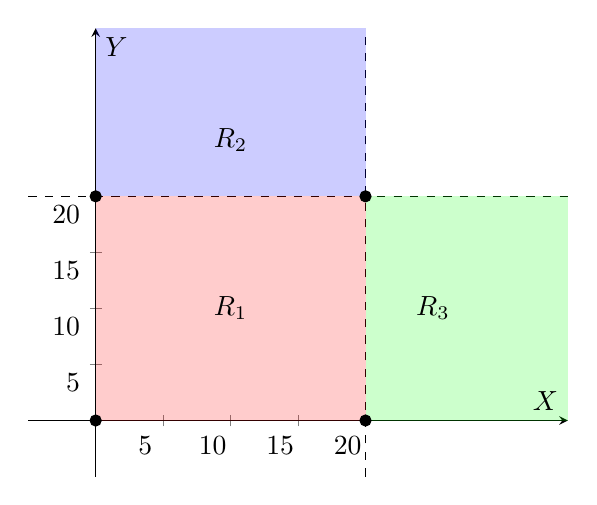
\begin{tikzpicture}
            \begin{axis}[
                axis lines = center,
                xlabel = $X$,
                ylabel = $Y$,
                xmin = -5, xmax = 35,
                ymin = -5, ymax = 35,
                xtick = {0,5,10,15,20},
                ytick = {0,5,10,15,20},
                yticklabel style = {yshift=-1.5ex},
                xticklabel style = {xshift=-1.5ex},
            ]
                \addplot[only marks] coordinates {
                    (0,0) (20,0) (0,20) (20,20)
                };

                % Líneas verticales
                \foreach \x in {20} {
                    \addplot[dashed] coordinates {(\x, -5) (\x, 35)};
                }

                % Líneas horizontales
                \foreach \y in {20} {
                    \addplot[dashed] coordinates {(-5, \y) (35, \y)};
                }                

                % Coloreamos cada una de las zonas
                \fill[red, opacity=0.2] (0,0) -- (20,0) -- (20,20) -- (0,20) -- cycle;
                \fill[blue, opacity=0.2] (0,20) -- (0,35) -- (20,35) -- (20,20) -- cycle;
                \fill[green, opacity=0.2] (20,0) -- (20,20) -- (35,20) -- (35,0) -- cycle;

                % Damos nombres a cada una de las zonas formadas
                \node at (10,10) {$R_1$};
                \node at (10,25) {$R_2$};
                \node at (25,10) {$R_3$};
            \end{axis}
        \end{tikzpicture}
    \end{figure}

    La función de distribución es:
    \begin{equation*}
        F_{(X,Y)}(x, y) = \int_{-\infty}^x \int_{-\infty}^y f(u, v) \, du \, dv
    \end{equation*}

    Estudiemos cada región por separado:
    \begin{itemize}
        \item \ul{Para $x\leq 0$ o $y\leq 0$}:
        
        Tenemos que $f(u, v) = 0$ para $u\leq x$ o $v\leq y$, por lo que:
        \begin{equation*}
            F_{(X,Y)}(x, y) = \int_{-\infty}^x \int_{-\infty}^y f(u, v) \, du \, dv =
            \int_{-\infty}^x \int_{-\infty}^y 0 \, du \, dv = 0.
        \end{equation*}

        \item \ul{Para $0 < x < 20$ y $0 < y < 20$} (región $R_1$):
        
        Tenemos que:
        \begin{equation*}
            F_{(X,Y)}(x, y) = \int_{-\infty}^x \int_{-\infty}^y f(u, v) \, du \, dv =
            \int_{0}^x \int_{0}^y \frac{1}{400} \, du \, dv = \frac{xy}{400}.
        \end{equation*}

        \item \ul{Para $0 < x < 20$ y $y \geq 20$} (región $R_2$):
        
        Tenemos que:
        \begin{equation*}
            F_{(X,Y)}(x, y) = \int_{-\infty}^x \int_{-\infty}^y f(u, v) \, du \, dv =
            \int_{0}^x \int_{0}^{20} \frac{1}{400} \, du \, dv = \frac{20x}{400} = \frac{x}{20}.
        \end{equation*}

        \item \ul{Para $x \geq 20$ y $0 < y < 20$} (región $R_3$):
        
        Tenemos que:
        \begin{equation*}
            F_{(X,Y)}(x, y) = \int_{-\infty}^x \int_{-\infty}^y f(u, v) \, du \, dv =
            \int_{0}^{20} \int_{0}^y \frac{1}{400} \, du \, dv = \frac{20y}{400} = \frac{y}{20}.
        \end{equation*}

        \item \ul{Para $x \geq 20$ y $y \geq 20$}:
        
        Tenemos que:
        \begin{equation*}
            F_{(X,Y)}(x, y) = \int_{-\infty}^x \int_{-\infty}^y f(u, v) \, du \, dv =
            \int_{0}^{20} \int_{0}^{20} \frac{1}{400} \, du \, dv = \frac{400}{400} = 1.
        \end{equation*}
    \end{itemize}

    Por tanto, la función de distribución es:
    \begin{equation*}
        F_{(X,Y)}(x, y) = \begin{cases}
            0, & x\leq 0 \text{ o } y\leq 0, \\
            \frac{xy}{400}, & 0 < x < 20 \text{ y } 0 < y < 20, \\
            \frac{x}{20}, & 0 < x < 20 \text{ y } y\geq 20, \\
            \frac{y}{20}, & x\geq 20 \text{ y } 0 < y < 20, \\
            1, & x\geq 20 \text{ y } y\geq 20.
        \end{cases}
    \end{equation*}

    Buscamos ahora la probabilidad de que en un día se vendan entre naranjas y manzanas, menos de 20 kilogramos. Para ello, buscamos la región del plano que cumple con la condición $X+Y < 20$. Tras representar la recta $y=20-x$,
    nos quedaremos con la región que queda por debajo de esta recta:
    \begin{figure}[H]
        \centering
        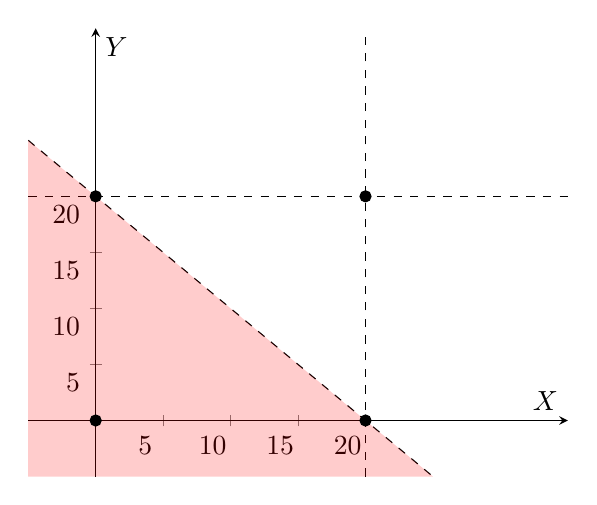
\begin{tikzpicture}
            \begin{axis}[
                axis lines = center,
                xlabel = $X$,
                ylabel = $Y$,
                xmin = -5, xmax = 35,
                ymin = -5, ymax = 35,
                xtick = {0,5,10,15,20},
                ytick = {0,5,10,15,20},
                yticklabel style = {yshift=-1.5ex},
                xticklabel style = {xshift=-1.5ex},
            ]
                \addplot[only marks] coordinates {
                    (0,0) (20,0) (0,20) (20,20)
                };

                % Líneas verticales
                \foreach \x in {20} {
                    \addplot[dashed] coordinates {(\x, -5) (\x, 35)};
                }

                % Líneas horizontales
                \foreach \y in {20} {
                    \addplot[dashed] coordinates {(-5, \y) (35, \y)};
                }

                % Representamos la recta y=20-x
                \addplot[domain=-5:35, samples=2, dashed] {20-x};

                % Coloreamos la región entre el (-5, 25), (25, -5) y (-5,-5)
                \fill[red, opacity=0.2] (-5,25) -- (25,-5) -- (-5,-5) -- cycle;
            \end{axis}
        \end{tikzpicture}
    \end{figure}

    Por tanto, tenemos que $P[X+Y < 20]$ es la integral de la función de densidad en la región coloreada, $R=\{(x,y)\in \mathbb{R}^2; x+y<20\}$:
    \begin{align*}
        P[X+Y < 20] &= \int_{-\infty}^{+\infty} \int_{-\infty}^{20-x} f(x, y) \, dy \, dx = \int_{0}^{20} \int_{0}^{20-x} \frac{1}{400} \, dy \, dx =\\&= \int_{0}^{20} \frac{20-x}{400} \, dx = \frac{1}{400}\left[20x-\frac{x^2}{2}\right]_0^{20} = \frac{1}{400}\left[400-200\right] = \frac{1}{2}.
    \end{align*}
\end{ejercicio}

\begin{ejercicio}
    La renta, $X$, y el consumo, $Y$, de los habitantes de una población, tienen por funciones de densidad
    \[
        f_X(x) = 2-2x; \quad 0 < x < 1; \quad f_{Y\mid X} (y\mid x) = \frac{1}{x}; \quad 0 < y < x.
    \]
    Determinar la función de densidad conjunta del vector aleatorio $(X,Y)$ y la probabilidad de que el consumo sea inferior a la mitad de la renta.\\

    Tenemos que, para $R=\{(x,y)\in \mathbb{R}^2; 0<x<1, 0<y<x\}$, la función de densidad conjunta es:
    \begin{equation*}
        f_{Y\mid X} (y\mid x) = \dfrac{f_{(X,Y)}(x, y)}{f_X(x)} \Longrightarrow f_{(X,Y)}(x, y) = f_X(x) \cdot f_{Y\mid X} (y\mid x) = (2-2x) \cdot \dfrac{1}{x} = \dfrac{2-2x}{x}.
    \end{equation*}

    Tenemos ahora que:
    \begin{align*}
        P[Y < \nicefrac{X}{2}] &= \int_{-\infty}^{+\infty} \int_{-\infty}^{\nicefrac{x}{2}} f_{(X,Y)}(x, y) \, dy \, dx = \int_{0}^{1} \int_{0}^{\nicefrac{x}{2}} \dfrac{2-2x}{x} \, dy \, dx =\\&= \int_{0}^{1} \dfrac{2-2x}{x}\cdot \dfrac{x}{2} \, dx = \int_{0}^{1} 1-x \, dx = \left[x-\dfrac{x^2}{2}\right]_0^1 = 1-\dfrac{1}{2} = \dfrac{1}{2}.
    \end{align*}

    
\end{ejercicio}

\begin{ejercicio}
    Una gasolinera tiene $Y$ miles de litros en su depósito de gasóleo al comienzo de cada semana. A lo largo de una semana se venden $X$ miles de litros del citado combustible, siendo la función de densidad conjunta de $(X,Y)$ :
    \[
        f(x, y) = \frac{1}{8}; \quad 0 < x < y < 4.
    \]
    Se pide:
    \begin{enumerate}
        \item Probar que $f(x, y)$ es función de densidad y obtener la función de distribución.
        
        En primer lugar, vemos que es no negativa. Veamos si es integrable:
        \begin{align*}
            \int_{-\infty}^{+\infty} \int_{-\infty}^{+\infty} f(x, y) \, dx \, dy &= \int_{0}^{4} \int_{x}^{4} \frac{1}{8} \, dy \, dx = \frac{1}{8}\int_{0}^{4} 4-x \, dx =\\&= \frac{1}{8}\left[4x-\frac{x^2}{2}\right]_0^4 = \frac{1}{8}\left[16-8\right] = 1.
        \end{align*}

        Tenemos por tanto que sí se trata de una función de densidad.
        Para obtener la función de distribución, representemos el conjunto en el que la función de densidad es no nula:
        \begin{figure}[H]
            \centering
            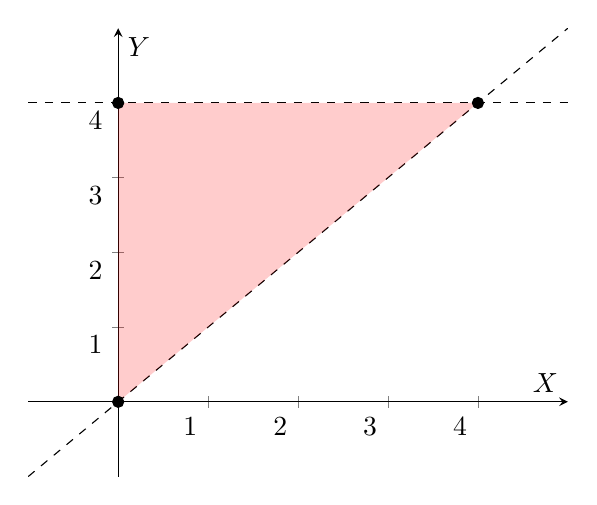
\begin{tikzpicture}
                \begin{axis}[
                    axis lines = center,
                    xlabel = $X$,
                    ylabel = $Y$,
                    xmin = -1, xmax = 5,
                    ymin = -1, ymax = 5,
                    xtick = {0,1,2,3,4},
                    ytick = {0,1,2,3,4},
                    yticklabel style = {yshift=-1.5ex},
                    xticklabel style = {xshift=-1.5ex},
                ]
                    \addplot[only marks] coordinates {
                        (0,0) (0,4) (4,4)
                    };

                    % Líneas horizontales
                    \foreach \y in {4} {
                        \addplot[dashed] coordinates {(-1, \y) (5, \y)};
                    }

                    % Representamos la recta y=x
                    \addplot[domain=-1:5, samples=2, dashed] {x};

                    % Coloreamos la región entre el (0,0), (0,4), (4,4)
                    \fill[red, opacity=0.2] (0,0) -- (0,4) -- (4,4) -- cycle;
                \end{axis}
            \end{tikzpicture}
        \end{figure}

        Para obtener la función de distribución, distinguimos casos:
        \begin{itemize}
            \item \ul{Para $x< 0$ o $y< 0$}:
            \begin{equation*}
                F_{(X,Y)}(x, y) = \int_{-\infty}^x \int_{-\infty}^y f(u, v) \, du \, dv = 0.
            \end{equation*}

            \item \ul{Para $0 < x < y <4$}:
            \begin{align*}
                F_{(X,Y)}(x, y) &= \int_{-\infty}^x \int_{-\infty}^y f(u, v) \, dv \, du = \int_{0}^x \int_{u}^y \frac{1}{8} \, dv \, du = \dfrac{1}{8}\int_{0}^x y-u \, du =\\&= \dfrac{1}{8}\left[yu-\dfrac{u^2}{2}\right]_0^x = \dfrac{1}{8}\left[xy-\dfrac{x^2}{2}\right]
                = \dfrac{2xy-x^2}{16}.
            \end{align*}

            \item \ul{Para $0 < x < 4$ y $y \geq 4$}:
            \begin{align*}
                F_{(X,Y)}(x, y) &= \int_{-\infty}^x \int_{-\infty}^y f(u, v) \, dv \, du =
                \int_0^x \int_u^4 \frac{1}{8} \, dv \, du = \dfrac{1}{8}\int_0^x 4-u \, du =\\&= \dfrac{1}{8}\left[4u-\dfrac{u^2}{2}\right]_0^x = \dfrac{1}{8}\left[4x-\dfrac{x^2}{2}\right] = \dfrac{8x-x^2}{16}.
            \end{align*}

            \item \ul{Para $x\geq y$ y $0\leq y<4$}:
            \begin{align*}
                F_{(X,Y)}(x, y) &= \int_{-\infty}^x \int_{-\infty}^y f(u, v) \, dv \, du =
                \int_0^{y} \int_{0}^v \frac{1}{8} \, du \, dv = \dfrac{1}{8}\int_0^y v \, dv =\\&= \dfrac{1}{8}\left[\dfrac{v^2}{2}\right]_0^y = \dfrac{1}{8}\cdot \dfrac{y^2}{2} = \dfrac{y^2}{16}.
            \end{align*}

            \item \ul{Para $x \geq 4$ y $y \geq 4$}:
            
            Hemos visto anteriormente que $F_{(X,Y)}(x,y) = 1$.
        \end{itemize}

        Por tanto,
        \begin{equation*}
            F_{(X,Y)}(x, y) = \begin{cases}
                0, & x<0 \text{ o } y<0, \\
                \dfrac{2xy-x^2}{16}, & 0 < x < y < 4, \\
                \dfrac{8x-x^2}{16}, & 0 < x < 4 \text{ y } y\geq 4, \\
                \dfrac{y^2}{16}, & x\geq y \text{ y } 0 \leq y < 4, \\
                1, & x\geq 4 \text{ y } y\geq 4.
            \end{cases}
        \end{equation*}

        

        \item Probabilidad de que en una semana se venda más de la tercera parte de los litros de que se dispone al comienzo de la misma.
        
        En este caso, nos piden calcular $P[X > \nicefrac{Y}{3}]$. Para ello, representamos la recta $y=3x$ y nos quedamos con la región que queda por encima de esta recta:
        \begin{figure}[H]
            \centering
            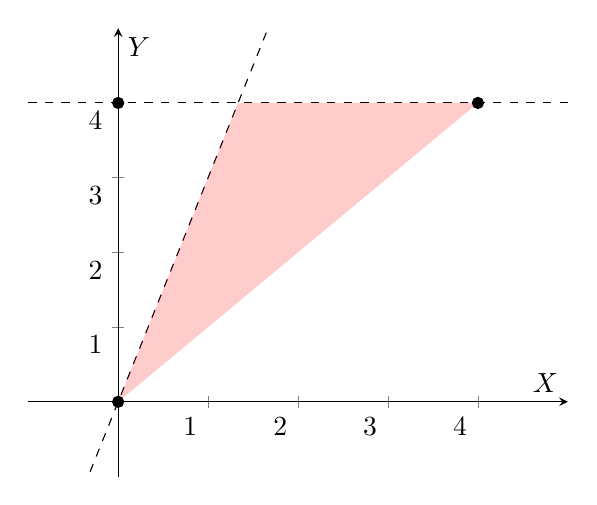
\begin{tikzpicture}
                \begin{axis}[
                    axis lines = center,
                    xlabel = $X$,
                    ylabel = $Y$,
                    xmin = -1, xmax = 5,
                    ymin = -1, ymax = 5,
                    xtick = {0,1,2,3,4},
                    ytick = {0,1,2,3,4},
                    yticklabel style = {yshift=-1.5ex},
                    xticklabel style = {xshift=-1.5ex},
                ]
                    \addplot[only marks] coordinates {
                        (0,0) (0,4) (4,4)
                    };

                    % Líneas horizontales
                    \foreach \y in {4} {
                        \addplot[dashed] coordinates {(-1, \y) (5, \y)};
                    }

                    % Representamos la recta y=3x
                    \addplot[domain=-1:5, samples=2, dashed] {3*x};

                    % Coloreamos la región entre el (0,0), (0,4), (4,4)
                    \fill[red, opacity=0.2] (0,0) -- (4,4) -- (1.333,4) -- cycle;
                \end{axis}
            \end{tikzpicture}
        \end{figure}

        Tenemos que integrar $f(x, y)$ en la región coloreada:
        \begin{align*}
            P[X > \nicefrac{Y}{3}] &=
            \int_{0}^{\nicefrac{4}{3}}
            \int_{x}^{3x} \frac{1}{8} \, dy \, dx + \int_{\nicefrac{4}{3}}^{4}
            \int_{x}^{4} \frac{1}{8} \, dy \, dx =\\&=
            \int_{0}^{\nicefrac{4}{3}} \frac{3x-x}{8} \, dx + \int_{\nicefrac{4}{3}}^{4} \frac{4-x}{8} \, dx = \dfrac{1}{8}\int_{0}^{\nicefrac{4}{3}} 2x \, dx + \dfrac{1}{8}\int_{\nicefrac{4}{3}}^{4} 4-x \, dx =\\&=
            \dfrac{1}{8}\left[x^2\right]_0^{\nicefrac{4}{3}} + \dfrac{1}{8}\left[4x-\dfrac{x^2}{2}\right]_{\nicefrac{4}{3}}^4
            = \dfrac{1}{8}\left[\dfrac{16}{9}\right] + \dfrac{1}{8}\left[16-\dfrac{16}{2}-\dfrac{16}{3}+\dfrac{16}{18}\right]
            =\\&= \dfrac{2}{9} + \dfrac{4}{9} = \dfrac{6}{9} = \dfrac{2}{3}.
        \end{align*}
        \item Si en una semana se han vendido $3.000$ litros de gasóleo, ¿cuál es la probabilidad de que al comienzo de la semana hubiese entre $3.500$ y $3.750$ litros de combustible?\\
        
        En este caso, nos piden:
        \begin{equation*}
            P[3.5 < Y < 3.75 \mid X = 3] = \int_{3.5}^{3.75} f_{Y\mid X=3} (y) \, dy.
        \end{equation*}

        Veamos el valor de $f_{Y\mid X=3} (y)$:
        \begin{equation*}
            f_{Y\mid X=3} (y) = \dfrac{f_{(X,Y)}(3, y)}{f_X(3)}
        \end{equation*}

        Calculemos por tanto la marginal de $X$:
        \begin{equation*}
            f_X(x) = \int_{-\infty}^{+\infty} f(x, y) \, dy = \int_{x}^{4} \dfrac{1}{8} \, dy = \frac{1}{8}\left[y\right]_x^4 = \frac{4-x}{8}
        \end{equation*}

        Por tanto, tenemos que:
        \begin{equation*}
            f_{Y\mid X=3} (y) = \dfrac{f_{(X,Y)}(3, y)}{f_X(3)} = \dfrac{\nicefrac{1}{8}}{\nicefrac{1}{8}} = 1.
        \end{equation*}

        Por tanto, la probabilidad pedida es:
        \begin{equation*}
            P[3.5 < Y < 3.75 \mid X = 3] = \int_{3.5}^{3.75} 1 \, dy = \left[y\right]_{3.5}^{3.75} = 3.75-3.5 = 0.25.
        \end{equation*}

    \end{enumerate}
\end{ejercicio}

\begin{ejercicio}
    Sea $(X,Y)$ un vector aleatorio continuo con función de densidad
    \[
        f(x, y) = k, \quad (x, y) \in R,
    \]
    siendo $R$ el rombo de vértices $(3,0)$; $(0,2)$; $(-3,0)$; $(0,-2)$. Calcular $k$ para que $f$ sea una función de densidad. Hallar las distribuciones marginales y condicionadas.\\

    Representamos en el plano cartesiano el rombo $R$:
    \begin{figure}[H]
        \centering
        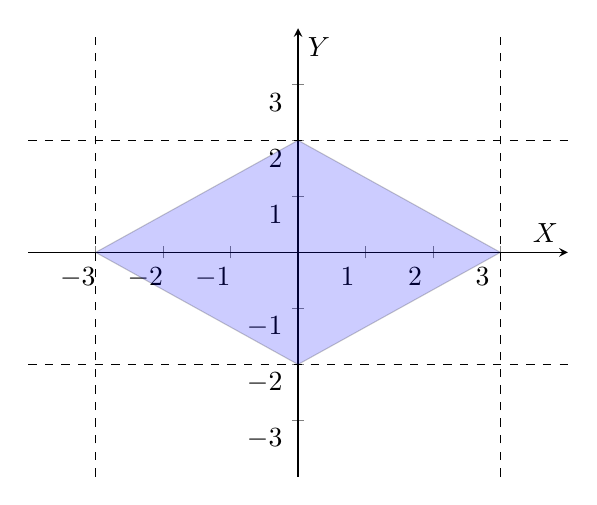
\begin{tikzpicture}
            \begin{axis}[
                axis lines = center,
                xlabel = $X$,
                ylabel = $Y$,
                xmin = -4, xmax = 4,
                ymin = -4, ymax = 4,
                xtick = {-3,-2,-1,0,1,2,3},
                ytick = {-3,-2,-1,0,1,2,3},
                yticklabel style = {yshift=-1.5ex},
                xticklabel style = {xshift=-1.5ex},
            ]
                \addplot[fill=blue, opacity=0.2] coordinates {
                    (3,0) (0,2) (-3,0) (0,-2)
                } --cycle;

                % Líneas horizontales
                \foreach \y in {2,-2} {
                    \addplot[dashed] coordinates {(-4, \y) (4, \y)};
                }

                % Líneas verticales
                \foreach \x in {-3,3} {
                    \addplot[dashed] coordinates {(\x, -4) (\x, 4)};
                }
            \end{axis}
        \end{tikzpicture}
    \end{figure}

    Para que $f$ sea una función de densidad, tenemos que:
    \begin{equation*}
        \int_{-\infty}^{+\infty} \int_{-\infty}^{+\infty} f(x, y) \, dx \, dy = 1.
    \end{equation*}

    Calculamos solo la integral en el primer cuadrante, ya que la función es simétrica. Para ello, calculamos la integral en el triángulo de vértices $(0,0)$; $(3,0)$; $(0,2)$. La recta que une los puntos $(3,0)$ y $(0,2)$ es $y=\nicefrac{-2}{3}x+2$. Por tanto, tenemos:
    \begin{align*}
        1&=\int_{-\infty}^{+\infty} \int_{-\infty}^{+\infty} f(x, y) \, dx \, dy
        = \int_R f(x, y) \, dx \, dy = 4\cdot \int_{0}^{3} \int_{0}^{\nicefrac{-2}{3}\cdot x+2} k \, dy \, dx =\\&= 4k\cdot \int_{0}^{3} \left[-\frac{2}{3}\cdot x+2\right] \, dx = 4k\cdot \left[-\frac{1}{3}\cdot x^2+2x\right]_0^3 = 4k\cdot \left[-\frac{1}{3}\cdot 9+6\right] = 4k\cdot \left[-3+6\right] = 12k.
    \end{align*}

    Por tanto, tenemos que $k=\nicefrac{1}{12}$. En este caso, vemos que además $f_{(X,Y)}$ es no negativa e integrable.\\

    Calculemos ahora la distribución marginal de $X$. Distinguimos:
    \begin{itemize}
        \item \ul{Si $x<-3$ o $x\geq 3$}:
        \begin{equation*}
            f_X(x) = \int_{-\infty}^{+\infty} f(x, y) \, dy = 0.
        \end{equation*}

        \item \ul{Si $-3\leq x<0$}:
    
        En este caso, tenemos que:
        \begin{equation*}
            -\dfrac{2}{3}\cdot x-2 \leq y \leq \dfrac{2}{3}\cdot x+2.
        \end{equation*}

        Por tanto, tenemos:
        \begin{align*}
            f_X(x) &= \int_{-\infty}^{+\infty} f(x, y) \, dy = \int_{\nicefrac{-2}{3}\cdot x-2}^{\nicefrac{2}{3}\cdot x+2} \frac{1}{12} \, dy = \frac{1}{12}\cdot \left[\nicefrac{2}{3}\cdot x+2-\left(\nicefrac{-2}{3}\cdot x-2\right)\right] =\\
            &= \frac{1}{12}\cdot \left[\frac{4}{3}\cdot x+4\right] = \dfrac{x}{9} + \dfrac{1}{3}.
        \end{align*}

        \item \ul{Si $0\leq x<3$}:
        
        En este caso, tenemos que:
        \begin{equation*}
            \frac{2}{3}\cdot x-2 \leq y \leq -\frac{2}{3}\cdot x+2.
        \end{equation*}

        Por tanto, tenemos:
        \begin{align*}
            f_X(x) &= \int_{-\infty}^{+\infty} f(x, y) \, dy = \int_{\nicefrac{2}{3}\cdot x-2}^{\nicefrac{-2}{3}\cdot x+2} \frac{1}{12} \, dy = \frac{1}{12}\cdot \left[\nicefrac{-2}{3}\cdot x+2-\left(\nicefrac{2}{3}\cdot x-2\right)\right] =\\
            &= \frac{1}{12}\cdot \left[-\frac{4}{3}\cdot x+4\right] = -\dfrac{x}{9} + \dfrac{1}{3}.
        \end{align*}
    \end{itemize}

    Por tanto, tenemos que:
    \begin{equation*}
        f_X(x) = \begin{cases}
            0, & x<-3 \text{ o } x\geq 3, \\
            \dfrac{x}{9} + \dfrac{1}{3}, & -3\leq x<0, \\
            -\dfrac{x}{9} + \dfrac{1}{3}, & 0\leq x<3.
        \end{cases}
    \end{equation*}

    Calculemos ahora la distribución marginal de $Y$. Distinguimos:
    \begin{itemize}
        \item \ul{Si $y<-2$ o $y\geq 2$}:
        \begin{equation*}
            f_Y(y) = \int_{-\infty}^{+\infty} f(x, y) \, dx = 0.
        \end{equation*}

        \item \ul{Si $-2\leq y<0$}:
    
        En este caso, tenemos que:
        \begin{equation*}
            -\frac{3}{2}\cdot y-3 \leq x \leq \frac{3}{2}\cdot y+3
        \end{equation*}

        Por tanto, tenemos:
        \begin{align*}
            f_Y(y) &= \int_{-\infty}^{+\infty} f(x, y) \, dx =
            \int_{\nicefrac{-3}{2}\cdot y-3}^{\nicefrac{3}{2}\cdot y+3} \frac{1}{12} \, dx = \frac{1}{12}\cdot \left[\nicefrac{3}{2}\cdot y+3-\left(\nicefrac{-3}{2}\cdot y-3\right)\right] =\\
            &= \dfrac{\nicefrac{y}{2}+1}{2} = \dfrac{y}{4} + \dfrac{1}{2}.
        \end{align*}

        \item \ul{Si $0\leq y<2$}:
        
        En este caso, tenemos que:
        \begin{equation*}
            \frac{3}{2}\cdot y-3 \leq x \leq -\frac{3}{2}\cdot y+3
        \end{equation*}

        Por tanto, tenemos:
        \begin{align*}
            f_Y(y) &= \int_{-\infty}^{+\infty} f(x, y) \, dx =
            \int_{\nicefrac{3}{2}\cdot y-3}^{\nicefrac{-3}{2}\cdot y+3} \frac{1}{12} \, dx = \frac{1}{12}\cdot \left[\nicefrac{-3}{2}\cdot y+3-\left(\nicefrac{3}{2}\cdot y-3\right)\right] =\\
            &= \dfrac{\nicefrac{-y}{2}+1}{2} = -\dfrac{y}{4} + \dfrac{1}{2}.
        \end{align*}
    \end{itemize}

    Por tanto, tenemos que:
    \begin{equation*}
        f_Y(y) = \begin{cases}
            0, & y<-2 \text{ o } y\geq 2, \\
            \dfrac{y}{4} + \dfrac{1}{2}, & -2\leq y<0, \\
            -\dfrac{y}{4} + \dfrac{1}{2}, & 0\leq y<2.
        \end{cases}
    \end{equation*}

    Calculemos ahora las distribuciones condicionadas.
    Dado $x^\ast\in \left]-3,3\right[$, tenemos:
    \begin{equation*}
        f_{Y\mid X=x^\ast} (y) = \dfrac{f_{(X,Y)}(x^\ast, y)}{f_X(x^\ast)}
        = \begin{cases}
            \dfrac{1}{12}\cdot \dfrac{1}{\nicefrac{x}{9} + \nicefrac{1}{3}}, & -3< x^\ast<0, \\
            \dfrac{1}{12}\cdot \dfrac{1}{\nicefrac{-x}{9} + \nicefrac{1}{3}}, & 0\leq x^\ast<3.
        \end{cases}
    \end{equation*}

    Por otro lado, dado $y^\ast\in \left]-2,2\right[$, tenemos que:
    \begin{equation*}
        f_{X\mid Y=y^\ast} (x) = \dfrac{f_{(X,Y)}(x, y^\ast)}{f_Y(y^\ast)}
        = \begin{cases}
            \dfrac{1}{12}\cdot \dfrac{1}{\nicefrac{y}{4} + \nicefrac{1}{2}}, & -2< y^\ast<0, \\
            \dfrac{1}{12}\cdot \dfrac{1}{\nicefrac{-y}{4} + \nicefrac{1}{2}}, & 0\leq y^\ast<2.
        \end{cases}
    \end{equation*}
\end{ejercicio}

\begin{ejercicio}
    Sea $(X,Y)$ un vector aleatorio continuo con función de densidad
    \[
        f(x, y) = k, \quad x^2 \leq y \leq 1,
    \]
    anulándose fuera del recinto indicado.
    \begin{enumerate}
        \item Hallar la constante $k$ para que $f$ sea una función de densidad.
        
        Representamos en el plano cartesiano el recinto en el que la función de densidad es no nula:
        \begin{figure}[H]
            \centering
            \begin{tikzpicture}
                \begin{axis}[
                    axis lines = center,
                    xlabel = $X$,
                    ylabel = $Y$,
                    xmin = -2, xmax = 2,
                    ymin = -0.5, ymax = 2,
                    xtick = {-1,0,1},
                    ytick = {-1,0,1},
                    yticklabel style = {yshift=-1.5ex},
                    xticklabel style = {xshift=-1.5ex},
                ]
                
                    % Dibuja la curva de y = x^2
                    \addplot [name path=A, blue, thick, forget plot, samples=70] {x^2};
                    
                    % Dibuja la línea horizontal en y=2
                    \addplot [name path=B, dashed, thick, forget plot] {1};
                
                    % Rellena el área bajo la curva entre x=0 y x=2
                    \addplot [
                        thick,
                        color=orange,
                        fill=orange,
                        fill opacity=0.4
                    ]
                    fill between [
                        of=A and B,
                        soft clip={domain=-1:1},
                    ];

                    % Coloreamos el área por debajo de A
                    \addplot [name path=C] {0};
                    \addplot [
                        thick,
                        color=red,
                        fill=red,
                        fill opacity=0.4
                    ]
                    fill between [
                        of=A and C,
                        soft clip={domain=-2:0},
                    ];

                    % Coloreamos el área por debajo de y=0
                    \addplot[fill=red, opacity=0.4] coordinates {
                        (-2, 0) (2,0) (2, -0.5) (-2, -0.5)
                    } --cycle;

                    % Coloreamos el área entre A y la recta x=-1
                    \addplot[name path=D] {3};
                    \addplot [
                        thick,
                        color=red,
                        fill=red,
                        fill opacity=0.4
                    ]
                    fill between [
                        of=D and A,
                        soft clip={domain=-2:-1},
                    ];

                    \addplot[fill=blue, opacity=0.2] coordinates {
                        (-1, 2) (-1, 1) (1,1) (1,2)
                    } --cycle;
                    
                    % Coloramos la zona R_4
                    \addplot [
                        thick,
                        color=green,
                        fill=green,
                        fill opacity=0.2
                    ]
                    fill between [
                        of=A and C,
                        soft clip={domain=0:1},
                    ];
                    \addplot[fill=green, opacity=0.2] coordinates {
                        (1,0) (1,1) (2,1) (2,0)
                    } --cycle;

                    \addplot[fill=olive, opacity=0.2] coordinates {
                        (1,1) (1,2) (2,2) (2,1)
                    } --cycle;


                    % Rectas verticales
                    \foreach \x in {-1,1} {
                        \addplot[dashed] coordinates {(\x, -0.5) (\x, 2)};
                    }

                    % Marcamos las zonas
                    \node at (-1.5, 0.5) {$R_1$};
                    \node at (0.3, 0.5) {$R_2$};
                    \node at (0.5, 1.5) {$R_3$};
                    \node at (1.5, 0.5) {$R_4$};
                    \node at (1.5, 1.5) {$R_5$};

                \end{axis}
            \end{tikzpicture}
        \end{figure}

        Para que $f$ sea una función de densidad, tenemos que:
        \begin{equation*}
            \int_{-\infty}^{+\infty} \int_{-\infty}^{+\infty} f(x, y) \, dx \, dy = 1.
        \end{equation*}

        Tenemos por tanto que:
        \begin{align*}
            1&=\int_{-\infty}^{+\infty} \int_{-\infty}^{+\infty} f(x, y) \, dx \, dy
            = \int_{-1}^{1} \int_{x^2}^{1} k \, dy \, dx = k\cdot \int_{-1}^{1} \left[y\right]_{x^2}^{1} \, dx = k\cdot \int_{-1}^{1} 1-x^2 \, dx =\\&= k\cdot \left[x-\dfrac{x^3}{3}\right]_{-1}^{1} = k\cdot \left[1-\dfrac{1}{3}-\left(-1+\dfrac{1}{3}\right)\right] = k\cdot \left[2-\dfrac{2}{3}\right] = \dfrac{4}{3}k
        \end{align*}
        Por tanto, tenemos que $k=\nicefrac{3}{4}$. En este caso, vemos que además $f_{(X,Y)}$ es no negativa e integrable.

        \item Calcular la función de distribución de probabilidad.
        
        Distinguimos casos:
        \begin{itemize}
            \item \ul{Si $x\leq -1$ \quad o \quad $y\leq 0$ \quad o \quad $x\in \left]-1,0\right[$ \text{ y } $y\leq x^2$} (zona $R_1$):
            \begin{equation*}
                F_{(X,Y)}(x, y) = \int_{-\infty}^x \int_{-\infty}^y f(u, v) \, du \, dv = 0.
            \end{equation*}

            \item \ul{Si $x^2\leq y\leq 1$} (zona $R_2$):
            \begin{align*}
                F_{(X,Y)}(x, y) &= \int_{-\infty}^x \int_{-\infty}^y f(u, v) \, dv \, du = \int_{-\sqrt{y}}^x \int_{u^2}^y \frac{3}{4} \, dv \, du = \frac{3}{4}\int_{-\sqrt{y}}^x \left[y-u^2\right] \, du =\\&= \frac{3}{4}\left[yu-\dfrac{u^3}{3}\right]_{-\sqrt{y}}^x = \frac{3}{4}\left[xy-\dfrac{x^3}{3}+y\sqrt{y}-\dfrac{y^{\nicefrac{3}{2}}}{3}\right] =\\
                &= \frac{3}{4}\left[xy-\dfrac{x^3}{3}+\dfrac{2}{3}\cdot y\sqrt{y}\right].
            \end{align*}

            \item \ul{Si $y\geq 1$ y $x\in \left]-1,1\right[$} (zona $R_3$):
            \begin{align*}
                F_{(X,Y)}(x, y) &= \int_{-\infty}^x \int_{-\infty}^y f(u, v) \, dv \, du = \int_{-1}^x \int_{u^2}^1 \frac{3}{4} \, dv \, du = \frac{3}{4}\int_{-1}^x \left[1-u^2\right] \, du =\\&= \frac{3}{4}\left[u-\dfrac{u^3}{3}\right]_{-1}^x = \frac{3}{4}\left[x-\dfrac{x^3}{3}+1-\dfrac{1}{3}\right] = \frac{3}{4}\left[x-\dfrac{x^3}{3}+\dfrac{2}{3}\right].
            \end{align*}

            \item \ul{Si $x\in \left]0,1\right[$ \text{ y } $0\leq y\leq x^2$ \quad o \quad $x\in \left]1,+\infty\right[$ \text{ y } $y\in ]0,1[$} (zona $R_4$):
            \begin{align*}
                F_{(X,Y)}(x, y) &= \int_{-\infty}^x \int_{-\infty}^y f(u, v) \, dv \, du = \int_{-\sqrt{y}}^{\sqrt{y}} \int_{u^2}^y \frac{3}{4} \, dv \, du = \frac{3}{4}\int_{-\sqrt{y}}^{\sqrt{y}} \left[y-u^2\right] \, du =\\&= \frac{3}{4}\left[yu-\dfrac{u^3}{3}\right]_{-\sqrt{y}}^{\sqrt{y}} = \frac{3}{4}\left[y\sqrt{y}-\dfrac{y^{\nicefrac{3}{2}}}{3}+y\sqrt{y}-\dfrac{y^{\nicefrac{3}{2}}}{3}\right] = y\sqrt{y}
            \end{align*}

            \item \ul{Si $x\geq 1$ y $y\geq 1$} (zona $R_5$):
            \begin{equation*}
                F_{(X,Y)}(x, y) = 1.
            \end{equation*}
        \end{itemize}

        Por tanto, tenemos que:
        \begin{equation*}
            F_{(X,Y)}(x, y) = \begin{cases}
                0, & x\leq -1 \text{ o } y\leq 0 \text{ o } x\in \left]-1,0\right[ \text{ y } y\leq x^2, \\
                \dfrac{3}{4}\left[xy-\dfrac{x^3}{3}+\dfrac{2}{3}\cdot y\sqrt{y}\right], & x^2\leq y\leq 1, \\
                \dfrac{3}{4}\left[x-\dfrac{x^3}{3}+\dfrac{2}{3}\right], & y\geq 1 \text{ y } x\in \left]-1,1\right[, \\
                y\sqrt{y}, & x\in \left]0,1\right[ \text{ y } 0\leq y\leq x^2 \text{ o } x>1\text{ y } y\in ]0,1[, \\
                1, & x\geq 1 \text{ y } y\geq 1.
            \end{cases}
        \end{equation*}

        \item Calcular $P(X \geq Y)$.
        
        Para calcular $P(X \geq Y)$, representamos la recta $y=x$ y nos quedamos con la región que queda por debajo de esta recta. Tenemos entonces que:
        \begin{align*}
            P(X \geq Y) &= \int_{0}^{1} \int_{x^2}^{x} \dfrac{3}{4} \, dy \, dx = \dfrac{3}{4}\int_{0}^{1} \left[x-x^2\right]\, dx = 
            \dfrac{3}{4}\left[\dfrac{x^2}{2} -\dfrac{x^3}{3}\right]_0^1 =\\&= \dfrac{3}{4}\left[\dfrac{1}{2}-\dfrac{1}{3}\right] = \dfrac{3}{4}\left[\dfrac{3-2}{6}\right] = \dfrac{3}{4}\left[\dfrac{1}{6}\right] = \dfrac{1}{8}.
        \end{align*}
        \item Calcular las distribuciones marginales.
        
        Para $x\in \left]-1,1\right[$, tenemos que:
        \begin{align*}
            f_X(x) &= \int_{-\infty}^{+\infty} f(x, y) \, dy = \int_{x^2}^{1} \dfrac{3}{4} \, dy = \dfrac{3}{4}\left[y\right]_{x^2}^1 = \dfrac{3}{4}\left[1-x^2\right].
        \end{align*}

        Para $y\in \left]0,1\right[$, tenemos que:
        \begin{align*}
            f_Y(y) &= \int_{-\infty}^{+\infty} f(x, y) \, dx = \int_{-\sqrt{y}}^{\sqrt{y}} \dfrac{3}{4} \, dx = \dfrac{3}{4}\left[x\right]_{-\sqrt{y}}^{\sqrt{y}} = \dfrac{3}{4}\left[\sqrt{y}+\sqrt{y}\right] = \dfrac{3}{2}\sqrt{y}.
        \end{align*}
        \item Calcular las distribuciones condicionadas.
        
        Dado $x^\ast\in \left]-1,1\right[$, tenemos que:
        \begin{equation*}
            f_{Y\mid X=x^\ast} (y) = \dfrac{f_{(X,Y)}(x^\ast, y)}{f_X(x^\ast)} = \dfrac{\nicefrac{3}{4}}{\nicefrac{3}{4}\left[1-(x^\ast)^2\right]} = \dfrac{1}{1-(x^\ast)^2}.
        \end{equation*}

        Dado $y^\ast\in \left]0,1\right[$, tenemos que:
        \begin{equation*}
            f_{X\mid Y=y^\ast} (x) = \dfrac{f_{(X,Y)}(x, y^\ast)}{f_Y(y^\ast)} = \dfrac{\nicefrac{3}{4}}{\nicefrac{3}{2}\sqrt{y^\ast}} = \dfrac{1}{2\sqrt{y^\ast}}.
        \end{equation*}
    \end{enumerate}

\end{ejercicio}

\begin{ejercicio}
    Sea $k\in \bb{R}$. Consideramos la función de densidad de probabilidad
    \[
        f(x, y) = \begin{cases}
            k\left[\frac{xy}{2}+1\right], & 0 < x < 1, -1 < y < 1, \\
            0, & \text{en otro caso}.
        \end{cases}
    \]
    Calcular:
    \begin{enumerate}
        \item La constante $k$ para que $f$ sea una función de densidad.
        
        Para que $f$ sea una función de densidad, tenemos que:
        \begin{equation*}
            \int_{-\infty}^{+\infty} \int_{-\infty}^{+\infty} f(x, y) \, dx \, dy = 1.
        \end{equation*}

        Tenemos por tanto que:
        \begin{align*}
            1&=\int_{-\infty}^{+\infty} \int_{-\infty}^{+\infty} f(x, y) \, dx \, dy
            = \int_{-1}^{1} \int_{0}^{1} k\left[\frac{xy}{2}+1\right] \, dx \, dy = k\int_{-1}^{1} \left[\dfrac{yx^2}{4}+x\right]_0^1
            =\\&= k\int_{-1}^{1} \left[\dfrac{y}{4}+1\right] \, dy = k\left[\dfrac{y^2}{8}+y\right]_{-1}^1 = k\left[\dfrac{1}{8}+1-\left(\dfrac{1}{8}-1\right)\right] = 2k \Longrightarrow k = \dfrac{1}{2}.
        \end{align*}

        Veamos ahora que, para dicho valor de $k$, $f$ es no negativa. Para ello, tenemos que:
        \begin{equation*}
            f(x, y) \geq 0 \Longleftrightarrow xy>-2 \Longleftrightarrow y>\dfrac{-2}{x}
        \end{equation*}
        Esto último es cierto, ya que $x\in ]0,1[$ e $y\in ]-1,1[$. Por tanto, $f$ es no negativa. Además, es integrable, por lo que $f$ es una función de densidad.

        \item La función de distribución de probabilidad.
        
        Representamos en el plano cartesiano la región en la que la función de densidad es no nula:
        \begin{figure}[H]
            \centering
            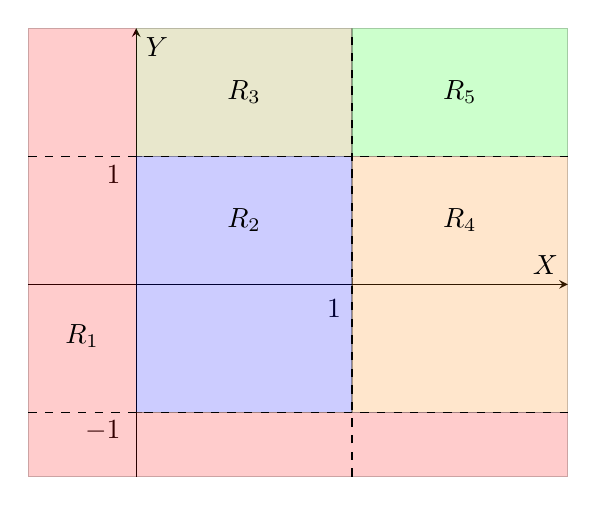
\begin{tikzpicture}
                \begin{axis}[
                    axis lines = center,
                    xlabel = $X$,
                    ylabel = $Y$,
                    xmin = -0.5, xmax = 2,
                    ymin = -1.5, ymax = 2,
                    xtick = {-1,0,1},
                    ytick = {-1,0,1},
                    yticklabel style = {yshift=-1.5ex},
                    xticklabel style = {xshift=-1.5ex},
                ]
                    \addplot[fill=red, opacity=0.2] coordinates {
                        (-0.5, -1.5) (-0.5,2) (0,2) (0,-1.5)
                    } --cycle;
                    \addplot[fill=red, opacity=0.2] coordinates {
                        (0, -1.5) (0, -1) (2,-1) (2,-1.5)
                    } --cycle;
                    \node at (-0.25, -0.4) {$R_1$};

                    \addplot[fill=blue, opacity=0.2] coordinates {
                        (0, -1) (1,-1) (1,1) (0,1)
                    } --cycle;
                    \node at (0.5, 0.5) {$R_2$};

                    \addplot[fill=olive, opacity=0.2] coordinates {
                        (0, 1) (1,1) (1,2) (0,2)
                    } --cycle;
                    \node at (0.5, 1.5) {$R_3$};

                    \addplot[fill=orange, opacity=0.2] coordinates {
                        (1,-1) (2,-1) (2,1) (1,1)
                    } --cycle;
                    \node at (1.5, 0.5) {$R_4$};

                    \addplot[fill=green, opacity=0.2] coordinates {
                        (1,1) (2,1) (2,2) (1,2)
                    } --cycle;
                    \node at (1.5, 1.5) {$R_5$};

                    % Líneas verticales
                    \foreach \x in {1} {
                        \addplot[dashed] coordinates {(\x, -1.5) (\x, 2)};
                    }

                    % Líneas horizontales
                    \foreach \y in {-1,1} {
                        \addplot[dashed] coordinates {(-0.5, \y) (2, \y)};
                    }
                \end{axis}
            \end{tikzpicture}
        \end{figure}

        Distinguimos casos:
        \begin{itemize}
            \item \ul{Si $x\leq 0 \qquad \text{o} \qquad y\leq -1$} (zona $R_1$):
            \begin{equation*}
                F_{(X,Y)}(x, y) = \int_{-\infty}^x \int_{-\infty}^y
                f(u, v) \, du \, dv = 0.
            \end{equation*}

            \item \ul{Si $x\in \left]0,1\right[ \text{ y } y\in \left]-1,1\right[$} (zona $R_2$):
            \begin{align*}
                F_{(X,Y)}(x, y) &= \int_{-\infty}^x \int_{-\infty}^y
                f(u, v) \, du \, dv = \int_{0}^x \int_{-1}^y
                \dfrac{1}{2}\left[\dfrac{uv}{2}+1\right] \, dv \, du =\\&= \int_{0}^x \left[\dfrac{uv^2}{8}+\frac{v}{2}\right]_{-1}^y \, du =
                \int_{0}^x \dfrac{uy^2}{8}+\frac{y}{2}-\dfrac{u}{8}+\dfrac{1}{2} \, du =\\&= \left[\dfrac{u^2y^2}{16}+\frac{y}{2}u-\dfrac{u^2}{16}+\dfrac{u}{2}\right]_0^x = \dfrac{x^2y^2}{16}+\frac{xy}{2}-\dfrac{x^2}{16}+\dfrac{x}{2}.
            \end{align*}

            \item \ul{Si $x\in \left]0,1\right[ \text{ y } y\geq 1$} (zona $R_3$):
            \begin{align*}
                F_{(X,Y)}(x, y) &= \int_{-\infty}^x \int_{-\infty}^y
                f(u, v) \, du \, dv = \int_{0}^x \int_{-1}^1
                \dfrac{1}{2}\left[\dfrac{uv}{2}+1\right] \, dv \, du =\\&= \int_{0}^x \left[\dfrac{uv^2}{8}+\frac{v}{2}\right]_{-1}^1 \, du =
                \int_{0}^x \dfrac{u}{8}+\dfrac{1}{2} - \left(\dfrac{u}{8}-\dfrac{1}{2}\right) \, du = \int_{0}^x 1 \, du = x.
            \end{align*}

            \item \ul{Si $y\in \left]-1,1\right[$ \text{ y } $x\geq 1$} (zona $R_4$):
            \begin{align*}
                F_{(X,Y)}(x, y) &= \int_{-\infty}^x \int_{-\infty}^y
                f(u, v) \, du \, dv = \int_{0}^1 \int_{-1}^y
                \dfrac{1}{2}\left[\dfrac{uv}{2}+1\right] \, dv \, du =\\&=
                \int_{0}^1 \left[\dfrac{uv^2}{8}+\frac{v}{2}\right]_{-1}^y \, du =
                \int_{0}^1 \dfrac{uy^2}{8}+\frac{y}{2}-\dfrac{u}{8}+\dfrac{1}{2} \, du =\\&=
                \left[\dfrac{u^2y^2}{16}+\frac{y}{2}u-\dfrac{u^2}{16}+\dfrac{u}{2}\right]_0^1 = \dfrac{y^2}{16}+\frac{y}{2}+\dfrac{7}{16}
            \end{align*}

            \item \ul{Si $y\geq 1$ \text{ y } $x\geq 1$} (zona $R_5$):
            \begin{equation*}
                F_{(X,Y)}(x, y) = 1.
            \end{equation*}
        \end{itemize}

        Por tanto, tenemos que:
        \begin{equation*}
            F_{(X,Y)}(x, y) = \begin{cases}
                0, & x\leq 0 \text{ o } y\leq -1, \\
                \dfrac{x^2y^2}{16}+\dfrac{xy}{2}-\dfrac{x^2}{16}+\dfrac{x}{2}, & x\in \left]0,1\right[ \text{ y } y\in \left]-1,1\right[, \\
                x, & x\in \left]0,1\right[ \text{ y } y\geq 1,\\
                \dfrac{y^2}{16}+\dfrac{y}{2}+\dfrac{7}{16}, & y\in \left]-1,1\right[ \text{ y } x\geq 1, \\
                1, & y\geq 1 \text{ y } x\geq 1.
            \end{cases}
        \end{equation*}
            

        \item Las distribuciones marginales.
        
        Para $x\in \left]0,1\right[$, tenemos que:
        \begin{align*}
            f_X(x) &= \int_{-\infty}^{+\infty} f(x, y) \, dy = \int_{-1}^{1} \dfrac{1}{2}\left[\dfrac{xy}{2}+1\right] \, dy = \dfrac{1}{2}\left[\dfrac{xy^2}{4}+y\right]_{-1}^1 = \dfrac{1}{2}\left[\dfrac{x}{4}+1-\dfrac{x}{4}+1\right] = 1
        \end{align*}

        Para $y\in \left]-1,1\right[$, tenemos que:
        \begin{align*}
            f_Y(y) &= \int_{-\infty}^{+\infty} f(x, y) \, dx = \int_{0}^{1} \dfrac{1}{2}\left[\dfrac{xy}{2}+1\right] \, dx = \dfrac{1}{2}\left[\dfrac{x^2y}{4}+x\right]_{0}^1 = \dfrac{1}{2}\left[\dfrac{y}{4}+1\right]
        \end{align*}
    \end{enumerate}
\end{ejercicio}

\begin{ejercicio}
    Sea $(X,Y)$ un vector aleatorio bidimensional continuo, con función de densidad de probabilidad
    \[
        f(x, y) = \begin{cases}
            k, & 0 < x + y < 1, |y| < 1, 0 < x < 1, \\
            0, & \text{en otro caso}.
        \end{cases}
    \]
    Responder a los siguientes apartados:
    \begin{enumerate}
        \item Hallar la constante $k$ para que $f$ sea una función de densidad de probabilidad.
        
        Para que $f$ sea una función de densidad, tenemos que:
        \begin{equation*}
            \int_{-\infty}^{+\infty} \int_{-\infty}^{+\infty} f(x, y) \, dx \, dy = 1.
        \end{equation*}

        Tenemos por tanto que:
        \begin{align*}
            1&=\int_{0}^{1} \int_{-x}^{1-x} k \, dx \, dy = k\int_{0}^{1} \left[y\right]_{-x}^{1-x} \, dx = k\int_{0}^{1} 1-x+x \, dx = k\int_{0}^{1} 1 \, dx = k
        \end{align*}

        Por tanto, tenemos que $k=1$. En este caso, vemos que además $f_{(X,Y)}$ es no negativa e integrable.

        \item Calcular la función de distribución de probabilidad.
        
        Dividimos el plano cartesiano en las distintas regiones:
        \begin{figure}[H]
            \centering
            \begin{tikzpicture}
                \begin{axis}[
                    axis lines = center,
                    xlabel = $X$,
                    ylabel = $Y$,
                    xmin = -1.5, xmax = 2,
                    ymin = -1.5, ymax = 2,
                    xtick = {-1,0,1},
                    ytick = {-1,0,1},
                    yticklabel style = {yshift=-1.5ex},
                    xticklabel style = {xshift=-1.5ex},
                ]
                    % Recta x+y=0
                    \addplot [name path=A, blue, thick, forget plot, samples=2] {-x};

                    % Recta x+y=1
                    \addplot [name path=B, blue, thick, forget plot, samples=2] {1-x};

                    % R1: Triangulo (0,1), (1,0), (0,0)
                    \addplot[fill=red, opacity=0.2] coordinates {
                        (0, 0) (1,0) (0,1)
                    } --cycle;
                    \node at (0.25, 0.25) {$R_1$};

                    % R2: Triangulo (1,0), (0,0), (1,-1)
                    \addplot[fill=blue, opacity=0.2] coordinates {
                        (1, 0) (0,0) (1,-1)
                    } --cycle;
                    \node at (0.75, -0.25) {$R_2$};

                    % R3: y<=0 y triángulo (0,0), (5,-5), (0,-5)
                    \addplot[fill=olive, opacity=0.2] coordinates {
                        (0, 0) (5,-5) (0,-5)
                    } --cycle;
                    \node at (0.5, -1) {$R_3$};
                    \addplot[fill=olive, opacity=0.2] coordinates {
                        (0, 5) (-5,5) (-5,-5) (0,-5)
                    } --cycle;
                    \addplot[fill=olive, opacity=0.2] coordinates {
                        (1, -1) (5,-1) (5, -5)
                    } --cycle;

                    % R4: Triangulo (1,0), (1,11), (0,1)
                    \addplot[fill=orange, opacity=0.2] coordinates {
                        (1, 0) (1,1) (0,1)
                    } --cycle;
                    \node at (0.75, 0.5) {$R_4$};

                    % R5: (0,1), (0,5), (1,5) y (1,1)
                    \addplot[fill=green, opacity=0.2] coordinates {
                        (0, 1) (0,5) (1,5) (1,1)
                    } --cycle;
                    \node at (0.5, 1.3) {$R_5$};

                    % R6: (1,1), (5,1), (5,0) y (1,0)
                    \addplot[fill=gray, opacity=0.2] coordinates {
                        (1, 1) (5,1) (5,0) (1,0)
                    } --cycle;
                    \node at (1.5, 0.5) {$R_6$};

                    % R7: (1,0), (1,-1), (5,-1) y (5,0)
                    \addplot[fill=yellow, opacity=0.2] coordinates {
                        (1, 0) (1,-1) (5,-1) (5,0)
                    } --cycle;
                    \node at (1.5, -0.5) {$R_7$};

                    % R8: (1,1), (1,5), (5,5) y (5,1)
                    \addplot[fill=pink, opacity=0.2] coordinates {
                        (1, 1) (1,5) (5,5) (5,1)
                    } --cycle;
                    \node at (1.5, 1.5) {$R_8$};                
                \end{axis}
            \end{tikzpicture}
        \end{figure}

        Distinguimos casos:
        \begin{itemize}
            \item \ul{Si $x\leq 0$ \quad o \quad $x+y\leq 0$} (zona $R_3$):
            \begin{equation*}
                F_{(X,Y)}(x, y) = \int_{-\infty}^x \int_{-\infty}^y f(u, v) \, du \, dv = 0.
            \end{equation*}

            \item \ul{Si $x\in \left]0,1\right[$ \quad y \quad $y\in \left]0,1\right[$ \quad y \quad $x+y\leq 1$} (zona $R_1$):
            \begin{align*}
                F_{(X,Y)}(x, y) &= \int_{-\infty}^x \int_{-\infty}^y f(u, v) \, dv \, du = \int_{0}^x \int_{-u}^y 1 \, dv \, du = \int_{0}^x \left[v\right]_{-u}^y \, du
                =\\&= \int_{0}^x y+u \, du = \left[yu+\dfrac{u^2}{2}\right]_0^x = xy+\dfrac{x^2}{2}.
            \end{align*}

            \item \ul{Si $x\in \left]0,1\right[$ \quad y \quad $y\in \left]-1,0\right[$ \quad y \quad $x+y\geq 0$} (zona $R_2$):
            \begin{align*}
                F_{(X,Y)}(x, y) &= \int_{-\infty}^x \int_{-\infty}^y f(u, v) \, du \, dv = \int_{-y}^x \int_{-u}^y 1 \, dv \, du = \int_{-y}^x \left[v\right]_{-u}^y \, du
                =\\&= \int_{-y}^x y+u \, du = \left[yu+\dfrac{u^2}{2}\right]_{-y}^x = xy+\dfrac{x^2}{2}-y(-y)-\dfrac{y^2}{2}
                =\\&= yx+\dfrac{x^2+y^2}{2}=\dfrac{(x+y)^2}{2}.
            \end{align*}

            \item \ul{Si $x\in \left]0,1\right[$ \quad y \quad $y\in \left]0,1\right[$ \quad y \quad $x+y\geq 1$} (zona $R_4$):
            \begin{align*}
                F_{(X,Y)}(x, y) &= \int_{-\infty}^x \int_{-\infty}^y f(u, v) \, du \, dv
                =\\&= \int_{0}^{1-y} \int_{0}^y 1 \, dv \, du
                + \int_{1-y}^x \int_{0}^{1-u} 1 \, dv \, du
                + \int_{0}^{x} \int_{-u}^0 1 \, dv \, du
                =\\&= \int_{0}^{1-y} y  \, du
                + \int_{1-y}^x 1-u \, du
                + \int_{0}^{x} u\, du
                =\\&= \left[yu\right]_0^{1-y}
                + \left[u-\dfrac{u^2}{2}\right]_{1-y}^x
                + \left[\dfrac{u^2}{2}\right]_0^x
                =\\&= y(1-y)+\left(x-\cancel{\dfrac{x^2}{2}}\right)-\left(1-y-\dfrac{(1-y)^2}{2}\right)+\cancel{\dfrac{x^2}{2}}
                =\\&= y-y^2+x-1+y+\dfrac{(1-y)^2}{2}
                = -(1-y)^2+x +\dfrac{(1-y)^2}{2}
                =\\&= x -\dfrac{(1-y)^2}{2}
            \end{align*}

            \item \ul{Si $x\in \left]0,1\right[$ \quad y \quad $y\in \left]1,\infty\right[$} (zona $R_5$):
            \begin{align*}
                F_{(X,Y)}(x, y) &= \int_{-\infty}^x \int_{-\infty}^y f(u, v) \, du \, dv
                = \int_{0}^{x} \int_{-u}^{1-u} 1 \, dv \, du
                =\\&= \int_{0}^{x} \left[v\right]_{-u}^{1-u} \, du
                = \int_{0}^{x} 1-u+u \, du
                = \int_{0}^{x} 1 \, du = x.
            \end{align*}

            \item \ul{Si $x\in \left]1,\infty\right[$ \quad y \quad $y\in \left]0,1\right[$} (zona $R_6$):
            \begin{align*}
                F_{(X,Y)}(x, y) &= \int_{-\infty}^x \int_{-\infty}^y f(u, v) \, du \, dv
                =\\&= \int_{0}^{1} \int_{-u}^{0} 1 \, dv \, du
                + \int_{0}^{1-y} \int_{0}^{y} 1 \, dv \, du
                + \int_{1-y}^{1} \int_{0}^{1-u} 1 \, dv \, du
                =\\&= \int_{0}^{1} u \, du
                + \int_{0}^{1-y} y \, du
                + \int_{1-y}^{1} 1-u \, du
                =\\&= \left[\dfrac{u^2}{2}\right]_0^1
                + \left[yu\right]_0^{1-y}
                + \left[u-\dfrac{u^2}{2}\right]_{1-y}^1
                =\\&= \cancel{\dfrac{1}{2}}+y(1-y)+1-\cancel{\dfrac{1}{2}}-\left[1-y-\dfrac{(1-y)^2}{2}\right]
                =\\&= y-y^2+y +\dfrac{(1-y)^2}{2}
                = 1-\dfrac{(1-y)^2}{2}
            \end{align*}

            \item \ul{Si $x\in \left]1,\infty\right[$ \quad y \quad $y\in \left]-1,0\right[$} (zona $R_7$):
            \begin{align*}
                F_{(X,Y)}(x, y) &= \int_{-\infty}^x \int_{-\infty}^y f(u, v) \, du \, dv
                =\\&= \int_{-y}^{1} \int_{-u}^{y} 1 \, dv \, du
                = \int_{-y}^{1} \left[v\right]_{-u}^{y} \, du
                = \int_{-y}^{1} y+u \, du
                =\\&= \left[yu+\dfrac{u^2}{2}\right]_{-y}^1
                = y+\dfrac{1}{2} + y^2-\dfrac{y^2}{2}
                = y+\dfrac{y^2+1}{2}
            \end{align*}

            \item \ul{Si $x\in \left]1,\infty\right[$ \quad y \quad $y\in \left]1,\infty\right[$} (zona $R_8$):
            \begin{align*}
                F_{(X,Y)}(x, y) &= \int_{-\infty}^x \int_{-\infty}^y f(u, v) \, du \, dv = 1
            \end{align*}
        \end{itemize}

        Por tanto, tenemos que:
        \begin{equation*}
            F_{(X,Y)}(x, y) = \begin{cases}
                0, & x\leq 0 \text{ o } x+y\leq 0,\ (R_3),\\
                xy+\dfrac{x^2}{2}, & x\in \left]0,1\right[ \text{ y } y\in \left]0,1\right[ \text{ y } x+y\leq 1,\ (R_1),\\
                \dfrac{(x+y)^2}{2}, & x\in \left]0,1\right[ \text{ y } y\in \left]-1,0\right[ \text{ y } x+y\geq 0,\ (R_2),\\
                x-\dfrac{(1-y)^2}{2}, & x\in \left]0,1\right[ \text{ y } y\in \left]0,1\right[ \text{ y } x+y\geq 1,\ (R_4),\\
                x, & x\in \left]0,1\right[ \text{ y } y\geq 1,\ (R_5),\\
                1-\dfrac{(1-y)^2}{2}, & x\in \left]1,\infty\right[ \text{ y } y\in \left]0,1\right[,\ (R_6),\\
                y+\dfrac{y^2+1}{2}, & x\in \left]1,\infty\right[ \text{ y } y\in \left]-1,0\right[,\ (R_7),\\
                1, & x\in \left]1,\infty\right[ \text{ y } y\geq 1,\ (R_8).
            \end{cases}
        \end{equation*}

        \item Calcular las distribuciones marginales.
        
        Para $x\in \left]0,1\right[$, ya que la función de densidad es constante, tenemos que:
        \begin{align*}
            f_X(x) &= \int_{-\infty}^{+\infty} f(x, y) \, dy = \int_{-x}^{1-x} 1 \, dy = \left[y\right]_{-x}^{1-x} = 1-x+x = 1.
        \end{align*}

        Para $y\in \left]0,1\right[$, ya que la función de densidad es constante, tenemos que:
        \begin{align*}
            f_Y(y) &= \int_{-\infty}^{+\infty} f(x, y) \, dx = \int_{0}^{1-y} 1 \, dx = \left[x\right]_{0}^{1-y} = 1-y.
        \end{align*}

        Para $y\in \left]-1,0\right[$, ya que la función de densidad es constante, tenemos que:
        \begin{align*}
            f_Y(y) &= \int_{-\infty}^{+\infty} f(x, y) \, dx = \int_{-y}^{1} 1 \, dx = \left[x\right]_{-y}^{1} = 1+y.
        \end{align*}

        Por tanto, tenemos que, para $y\in \left]-1,1\right[$:
        \begin{equation*}
            f_Y(y) = 1-|y|.
        \end{equation*}

        \item Calcular las distribuciones condicionadas.
        
        Dado $x^\ast\in \left]-1,1\right[$, tenemos para $y\in \left]0,1\right[$, $0<x^\ast + y < 1$:
        \begin{equation*}
            f_{Y\mid X=x^\ast} (y) = \dfrac{f_{(X,Y)}(x^\ast, y)}{f_X(x^\ast)} = \dfrac{1}{1} = 1.
        \end{equation*}

        Dado $y^\ast\in \left]-1,1\right[$, tenemos para $x\in \left]0,1\right[$, $0<x+y^\ast<1$:
        \begin{equation*}
            f_{X\mid Y=y^\ast} (x) = \dfrac{f_{(X,Y)}(x, y^\ast)}{f_Y(y^\ast)} = \dfrac{1}{1-|y^\ast|}.
        \end{equation*}
    \end{enumerate}
\end{ejercicio}

\begin{ejercicio}
    Sea $(X,Y)$ un vector aleatorio bidimensional continuo, con distribución de probabilidad uniforme sobre el triángulo de vértices $(0,0)$; $(0,1)$; $(1,1)$. Determinar:
    \begin{enumerate}
        \item La función de densidad de probabilidad.
        
        Veamos en primer lugar el triángulo en cuestión:
        \begin{figure}[H]
            \centering
            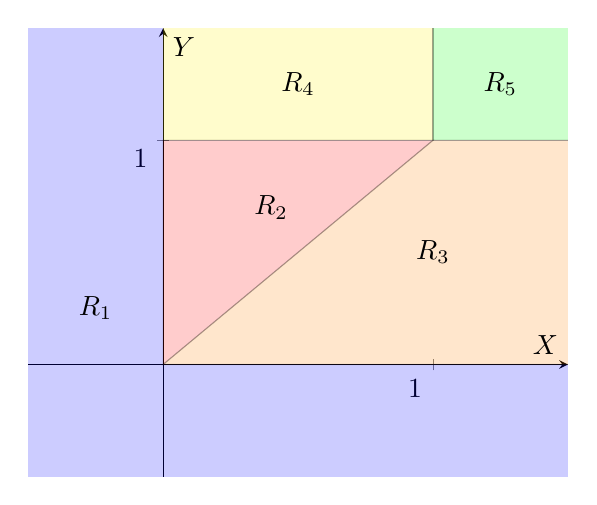
\begin{tikzpicture}
                \begin{axis}[
                    axis lines = center,
                    xlabel = $X$,
                    ylabel = $Y$,
                    xmin = -0.5, xmax = 1.5,
                    ymin = -0.5, ymax = 1.5,
                    xtick = {0,1},
                    ytick = {0,1},
                    yticklabel style = {yshift=-1.5ex},
                    xticklabel style = {xshift=-1.5ex},
                ]   
                    % R2
                    \addplot[fill=red, opacity=0.2] coordinates {
                        (0, 0) (0,1) (1,1)
                    } --cycle;
                    \node at (0.4, 0.7) {$R_2$};

                    % R1
                    \addplot[fill=blue, opacity=0.2] coordinates {
                        (-3, 3) (-3,-3) (3,-3)  (3,0) (0,0) (0,3)
                    } --cycle;
                    \node at (-0.25, 0.25) {$R_1$};

                    % R3
                    \addplot[fill=orange, opacity=0.2] coordinates {
                        (0,0) (1,1) (3,1)  (3,0)
                    } --cycle;
                    \node at (1, 0.5) {$R_3$};

                    % R4
                    \addplot[fill=yellow, opacity=0.2] coordinates {
                        (0,1) (1,1) (1,3) (0,3)
                    } --cycle;
                    \node at (0.5, 1.25) {$R_4$};

                    % R5
                    \addplot[fill=green, opacity=0.2] coordinates {
                        (1,1) (3,1) (3,3) (1,3)
                    } --cycle;
                    \node at (1.25, 1.25) {$R_5$};
                \end{axis}
            \end{tikzpicture}
        \end{figure}

        La función de densidad de probabilidad es constante, por lo que:
        \begin{equation*}
            f(x, y) = \begin{cases}
                k, & x\in [0,1], x\leq y\leq 1, \\
                0, & \text{en otro caso}.
            \end{cases}
        \end{equation*}

        Para que $f$ sea una función de densidad, tenemos que:
        \begin{align*}
            1&=\int_{-\infty}^{+\infty} \int_{-\infty}^{+\infty} f(x, y) \, dx \, dy = \int_{0}^{1} \int_{x}^{1} k \, dy \, dx = k\int_{0}^{1} \left[y\right]_{x}^{1} \, dx =\\&= k\int_{0}^{1} 1-x \, dx = k\left[x-\dfrac{x^2}{2}\right]_0^1 = k\left(1-\dfrac{1}{2}\right) = \dfrac{k}{2} \Longrightarrow k=2.
        \end{align*}
        \item La función de distribución de probabilidad.
        
        Distinguimos casos:
        \begin{itemize}
            \item \ul{Si $x\leq 0$ \quad o \quad $y\leq 0$} (zona $R_1$):
            \begin{equation*}
                F_{(X,Y)}(x, y) = \int_{-\infty}^x \int_{-\infty}^y f(u, v) \, du \, dv = 0.
            \end{equation*}

            \item \ul{Si $x\in \left]0,1\right[$ \quad y \quad $x<y<1$} (zona $R_2$):
            \begin{align*}
                F_{(X,Y)}(x, y) &= \int_{-\infty}^x \int_{-\infty}^y f(u, v) \, du \, dv = \int_{0}^x \int_{u}^y 2 \, dv \, du = \int_{0}^x 2(y-u) \, du
                =\\&= 2\left[yu-\dfrac{u^2}{2}\right]_0^x = 2\left(xy-\dfrac{x^2}{2}\right) = 2xy-x^2.
            \end{align*}

            \item \ul{Si $y\in \left]0,1,\infty\right[$ \quad y \quad $x>y$} (zona $R_3$):
            \begin{align*}
                F_{(X,Y)}(x, y) &= \int_{-\infty}^x \int_{-\infty}^y f(u, v) \, du \, dv = \int_{0}^{y} \int_{u}^{y} 2 \, dv \, du = \int_{0}^{y} 2(y-u) \, du
                =\\&= 2\left[yu-\dfrac{u^2}{2}\right]_0^y = 2\left(y^2-\dfrac{y^2}{2}\right) = 2\cdot \dfrac{y^2}{2} = y^2.
            \end{align*}

            \item \ul{Si $x\in \left]0,1\right[$ \quad y \quad $y\geq 1$} (zona $R_4$):
            \begin{align*}
                F_{(X,Y)}(x, y) &= \int_{-\infty}^x \int_{-\infty}^y f(u, v) \, du \, dv = \int_{0}^{x} \int_{u}^{1} 2 \, dv \, du = \int_{0}^{x} 2(1-u) \, du
                =\\&= 2\left[u-\dfrac{u^2}{2}\right]_0^x = 2\left(x-\dfrac{x^2}{2}\right) = 2x-x^2.
            \end{align*}

            \item \ul{Si $x,y\geq 1$} (zona $R_5$):
            \begin{equation*}
                F_{(X,Y)}(x, y) = 1.
            \end{equation*}
        \end{itemize}

        Por tanto, tenemos que:
        \begin{equation*}
            F_{(X,Y)}(x, y) = \begin{cases}
                0, & x\leq 0 \text{ o } y\leq 0, (R_1), \\
                2xy-x^2, & x\in \left]0,1\right[ \text{ y } x<y<1, (R_2), \\
                y^2, & y\in \left]0,1\right[ \text{ y } x>y, (R_3), \\
                2x-x^2, & x\in \left]0,1\right[ \text{ y } y\geq 1, (R_4), \\
                1, & x,y\geq 1, (R_5).
            \end{cases}
        \end{equation*}
        \item Las distribuciones marginales.
        
        Para $x\in \left]0,1\right[$, ya que la función de densidad es constante, tenemos que:
        \begin{align*}
            f_X(x) &= \int_{-\infty}^{+\infty} f(x, y) \, dy = \int_{x}^{1} 2 \, dy = 2\left[y\right]_{x}^{1} = 2(1-x).
        \end{align*}

        Para $y\in \left]0,1\right[$, ya que la función de densidad es constante, tenemos que:
        \begin{align*}
            f_Y(y) &= \int_{-\infty}^{+\infty} f(x, y) \, dx = \int_{0}^{y} 2 \, dx = 2\left[x\right]_{0}^{y} = 2y.
        \end{align*}
        \item Las distribuciones condicionadas.
        
        Dado $x^\ast\in \left]0,1\right[$, tenemos para $y\in \left]0,1\right[$, $x^\ast<y<1$:
        \begin{equation*}
            f_{Y\mid X=x^\ast} (y) = \dfrac{f_{(X,Y)}(x^\ast, y)}{f_X(x^\ast)} = \dfrac{2}{2(1-x^\ast)} = \dfrac{1}{1-x^\ast}.
        \end{equation*}

        Dado $y^\ast\in \left]0,1\right[$, tenemos para $x\in \left]0,1\right[$, $x<y^\ast<1$:
        \begin{equation*}
            f_{X\mid Y=y^\ast} (x) = \dfrac{f_{(X,Y)}(x, y^\ast)}{f_Y(y^\ast)} = \dfrac{2}{2y^\ast} = \dfrac{1}{y^\ast}.
        \end{equation*}
    \end{enumerate}
\end{ejercicio}

\begin{ejercicio}
    Sea $(X,Y)$ una variable aleatoria bidimensional con distribución uniforme en el recinto
    \[
        C = \{(x, y) \in \mathbb{R}^2; x^2 + y^2 < 1; x \geq 0, y \geq 0\}.
    \]
    Calcular:
    \begin{enumerate}
        \item La función de densidad conjunta.
        
        La función de densidad conjunta es constante, por lo que:
        \begin{equation*}
            f(x, y) = \begin{cases}
                k, & x^2+y^2<1, x,y\geq 0 \\
                0, & \text{en otro caso}.
            \end{cases}
        \end{equation*}

        Para que $f$ sea una función de densidad, tenemos que:
        \begin{align*}
            1&=\int_{-\infty}^{+\infty} \int_{-\infty}^{+\infty} f(x, y) \, dx \, dy
        \end{align*}

        Hay dos opciones:
        \begin{description}
            \item[Integrando de la forma usual:]
            
            Es necesario que:
            \begin{equation*}
                \int_{0}^{1} \int_{0}^{\sqrt{1-x^2}} k \, dy \, dx = k\int_{0}^{1} \sqrt{1-x^2} \, dx
            \end{equation*}

            Haciendo el cambio de variable $x=\sen(t)$, tenemos que:
            \begin{align*}
                1&=k\int_{0}^{\frac{\pi}{2}} \cos(t)\cos(t) \, dt = k\int_{0}^{\frac{\pi}{2}} \cos^2(t) \, dt
                = k\int_{0}^{\frac{\pi}{2}} \dfrac{1+\cos(2t)}{2} \, dt
                =\\&= k\left[\dfrac{t}{2}+\dfrac{\sen(2t)}{4}\right]_0^{\frac{\pi}{2}}
                = k\left[\dfrac{\pi}{4}\right] \Longrightarrow k=\dfrac{4}{\pi}.
            \end{align*}

            \item[Razonando la forma de $C$:]
            
            Sabemos que $C$ es un cuarto de círculo de radio 1, por lo que su área es $\nicefrac{\pi}{4}$. Por tanto, tenemos que:
            \begin{equation*}
                1=\int_C f(x, y) = k\int_C 1 = k\cdot \lm(C) = k\cdot \dfrac{\pi}{4} \Longrightarrow k=\dfrac{4}{\pi}.
            \end{equation*}
        \end{description}
        \item La función de distribución conjunta.
        
        Dividimos el plano cartesiano en las distintas regiones:
        \begin{figure}[H]
            \centering
            \begin{tikzpicture}
                \begin{axis}[
                    axis lines = center,
                    xlabel = $X$,
                    ylabel = $Y$,
                    xmin = -0.5, xmax = 1.5,
                    ymin = -0.5, ymax = 1.5,
                    xtick = {0,1},
                    ytick = {0,1},
                    yticklabel style = {yshift=-1.5ex},
                    xticklabel style = {xshift=-1.5ex},
                    axis equal,
                ]
                    % R2: Cuarto de circunferencia
                    \addplot [name path=A, blue, thick, forget plot, samples=70, domain=0:1] {sqrt(1-x^2)};
                    
                    % Dibuja la línea horizontal en y=0
                    \addplot [name path=B, forget plot, draw=none] {0};

                    % Dibuja la línea horizontal en y=0
                    \addplot [name path=C, forget plot, draw=none] {1};
                
                    % Rellena el área bajo la curva entre x=0 y x=1
                    \addplot [
                        thick,
                        color=orange,
                        fill=orange,
                        fill opacity=0.4
                    ]
                    fill between [
                        of=A and B,
                        soft clip={domain=0:1},
                    ];
                    
                    % Señalamos zona R2
                    \node at (0.5, 0.5) {$R_2$};

                    % R1: (0, 2), (-2, 2), (-2, -2), (2, -2), (2, 0), (0, 0)
                    \addplot[fill=red, opacity=0.2] coordinates {
                        (0, 2) (-2, 2) (-2, -2) (2, -2) (2, 0) (0, 0)
                    } --cycle;
                    \node at (-0.25, -0.25) {$R_1$};

                    \addplot [
                        thick,
                        color=teal,
                        fill=teal,
                        fill opacity=0.4
                    ]
                    fill between [
                        of=C and A,
                        soft clip={domain=0:1},
                    ];
                    \node at (0.8, 0.8) {$R_3$};

                    \addplot[fill=blue, opacity=0.2] coordinates {
                        (0, 1) (1,1) (1,2) (0,2)
                    } --cycle;
                    \node at (0.5, 1.25) {$R_4$};

                    \addplot[fill=green, opacity=0.2] coordinates {
                        (1, 1) (2,1) (2,0) (1,0)
                    } --cycle;
                    \node at (1.25, 0.5) {$R_5$};

                    \addplot[fill=olive, opacity=0.2] coordinates {
                        (1, 1) (2,1) (2,2) (1,2)
                    } --cycle;
                    \node at (1.25, 1.25) {$R_6$};
                \end{axis}
            \end{tikzpicture}
        \end{figure}

        Distinguimos casos:
        \begin{itemize}
            \item \ul{Si $x\leq 0$ \quad o \quad $y\leq 0$} (zona $R_1$):
            \begin{equation*}
                F_{(X,Y)}(x, y) = \int_{-\infty}^x \int_{-\infty}^y f(u, v) \, du \, dv = 0.
            \end{equation*}

            \item \ul{Si $x\in \left]0,1\right[$ \quad y \quad $y\in \left]0,\sqrt{1-x^2}\right[$} (zona $R_2$):
            \begin{align*}
                F_{(X,Y)}(x, y) &= \int_{-\infty}^x \int_{-\infty}^y f(u, v) \, dv \, du = \int_{0}^x \int_{0}^y \dfrac{4}{\pi} \, dv \, du = \int_{0}^x \dfrac{4}{\pi}y \, du
                =\\&= \dfrac{4}{\pi}\left[yu\right]_0^x = \dfrac{4}{\pi}\cdot xy
            \end{align*}

            \item \ul{Si $x\in \left]0,1\right[$ \quad y \quad $y\in \left]\sqrt{1-x^2},1\right[$} (zona $R_3$):
            \begin{align*}
                F_{(X,Y)}(x, y) &= \int_{-\infty}^x \int_{-\infty}^y f(u, v) \, dv \, du =\\&= \int_{0}^{\sqrt{1-y^2}}\int_0^y \dfrac{4}{\pi} \, dv \, du + \int_{\sqrt{1-y^2}}^x \int_0^{\sqrt{1-u^2}} \dfrac{4}{\pi} \, dv \, du =\\
                &= \int_{0}^{\sqrt{1-y^2}} \dfrac{4}{\pi}y \, du + \int_{\sqrt{1-y^2}}^x \dfrac{4}{\pi}\sqrt{1-u^2} \, du
            \end{align*}

            Para resolver la segunda integral, hacemos el cambio de variable dado por $u=\sen(t)$, $du=\cos(t)dt$:
            \begin{align*}
                F_{(X,Y)}(x, y) &= \dfrac{4}{\pi} y\sqrt{1-y^2} + \dfrac{4}{\pi}\int_{\arcsen(\sqrt{1-y^2})}^{\arcsen(x)} \cos^2(t) \, dt
                =\\&= \dfrac{4}{\pi} y\sqrt{1-y^2} + \dfrac{4}{\pi}\int_{\arcsen(\sqrt{1-y^2})}^{\arcsen(x)} \dfrac{1+\cos(2t)}{2} \, dt
                =\\&= \dfrac{4}{\pi} y\sqrt{1-y^2} + \dfrac{4}{\pi}\left[\dfrac{t}{2}+\dfrac{\sen(2t)}{4}\right]_{\arcsen(\sqrt{1-y^2})}^{\arcsen(x)}
                =\\&= \dfrac{4}{\pi} y\sqrt{1-y^2} + \dfrac{4}{\pi}\left[\dfrac{\arcsen(x)}{2}+\dfrac{\sen(2\arcsen(x))}{4}-\right.\\&\qquad -\left.\dfrac{\arcsen(\sqrt{1-y^2})}{2}-\dfrac{\sen(2\arcsen(\sqrt{1-y^2}))}{4}\right]
            \end{align*}

            Veamos cuánto vale anteriormente $\sen(2\arcsen(x))$ para cierto $x\in \bb{R}$:
            \begin{align*}
                \sen(2\arcsen(x)) &= 2\sen(\arcsen(x))\cos(\arcsen(x)) = 2x\sqrt{1-x^2}.
            \end{align*}

            Por tanto, tenemos que:
            \begin{align*}
                F_{(X,Y)}(x, y) &= \dfrac{4}{\pi} y\sqrt{1-y^2} + \dfrac{4}{\pi}\left[\dfrac{\arcsen(x)}{2}+\dfrac{2x\sqrt{1-x^2}}{4}-\right.\\&\qquad -\left.\dfrac{\arcsen(\sqrt{1-y^2})}{2}-\dfrac{2\sqrt{1-y^2}\sqrt{y^2}}{4}\right]
                =\\&= \dfrac{4}{\pi} y\sqrt{1-y^2} + \dfrac{2}{\pi}\arcsen(x)+\dfrac{2}{\pi}x\sqrt{1-x^2}-\\&\qquad-\dfrac{2}{\pi}\arcsen(\sqrt{1-y^2})-\dfrac{2}{\pi}y\sqrt{1-y^2}.
            \end{align*}

            \item \ul{Si $x\in \left]0,1\right[$ \quad y \quad $y\geq 1$} (zona $R_4$):
            \begin{align*}
                F_{(X,Y)}(x, y) &= \int_{-\infty}^x \int_{-\infty}^y f(u, v) \, dv \, du = \int_{0}^x \int_{0}^{\sqrt{1-u^2}} \dfrac{4}{\pi} \, dv \, du
                =\\&= \int_{0}^x \dfrac{4}{\pi}\sqrt{1-u^2} \, du
            \end{align*}

            Para resolver la integral, de nuevo hacemos el cambio de variable dado por $u=\sen(t)$, $du=\cos(t)dt$:
            \begin{align*}
                F_{(X,Y)}(x, y) &= \dfrac{4}{\pi}\int_{0}^{\arcsen(x)} \cos^2(t) \, dt
                =\\&= \dfrac{4}{\pi}\int_{0}^{\arcsen(x)} \dfrac{1+\cos(2t)}{2} \, dt
                =\\&= \dfrac{4}{\pi}\left[\dfrac{t}{2}+\dfrac{\sen(2t)}{4}\right]_0^{\arcsen(x)}
                =\\&= \dfrac{4}{\pi}\left[\dfrac{\arcsen(x)}{2}+\dfrac{\sen(2\arcsen(x))}{4}\right]
                =\\&= \dfrac{4}{\pi}\left[\dfrac{\arcsen(x)}{2}+\dfrac{2x\sqrt{1-x^2}}{4}\right]
                =\\&= \dfrac{2}{\pi}\arcsen(x)+\dfrac{2}{\pi}x\sqrt{1-x^2}.
            \end{align*}

            \item \ul{Si $y\in \left]0,1\right[$ \quad y \quad $x\geq 1$} (zona $R_5$):
            \begin{align*}
                F_{(X,Y)}(x, y) &= \int_{-\infty}^x \int_{-\infty}^y f(u, v) \, dv \, du =\\
                &= \int_{0}^{\sqrt{1-y^2}} \int_{0}^y \dfrac{4}{\pi} \, dv \, du + \int_{\sqrt{1-y^2}}^1 \int_{0}^{\sqrt{1-u^2}} \dfrac{4}{\pi} \, dv \, du
                =\\&= \int_{0}^{\sqrt{1-y^2}} \dfrac{4}{\pi}y \, du + \int_{\sqrt{1-y^2}}^1 \dfrac{4}{\pi}\sqrt{1-u^2} \, du
            \end{align*}

            Para resolver la segunda integral, de nuevo hacemos el cambio de variable dado por $u=\sen(t)$, $du=\cos(t)dt$:
            \begin{align*}
                F_{(X,Y)}(x, y) &= \dfrac{4}{\pi}y\left[u\right]_0^{\sqrt{1-y^2}} + \dfrac{4}{\pi}\int_{\arcsen(\sqrt{1-y^2})}^{\nicefrac{\pi}{2}} \cos^2(t) \, dt
                =\\&= \dfrac{4}{\pi}y\sqrt{1-y^2} + \dfrac{4}{\pi}\int_{\arcsen(\sqrt{1-y^2})}^{\nicefrac{\pi}{2}} \dfrac{1+\cos(2t)}{2} \, dt
                =\\&= \dfrac{4}{\pi}y\sqrt{1-y^2} + \dfrac{4}{\pi}\left[\dfrac{t}{2}+\dfrac{\sen(2t)}{4}\right]_{\arcsen(\sqrt{1-y^2})}^{\nicefrac{\pi}{2}}
                =\\&= \dfrac{4}{\pi}y\sqrt{1-y^2} + \dfrac{4}{\pi}\left[\dfrac{\nicefrac{\pi}{2}}{2}+\dfrac{\sen(\pi)}{4}-\dfrac{\arcsen(\sqrt{1-y^2})}{2}-\right.\\&\qquad\left.-\dfrac{\sen(2\arcsen(\sqrt{1-y^2}))}{4}\right]
                =\\&= \dfrac{4}{\pi}y\sqrt{1-y^2} + 1 - \dfrac{2}{\pi}\arcsen(\sqrt{1-y^2}) - \dfrac{2}{\pi}y\sqrt{1-y^2}
                =\\&= \dfrac{2}{\pi}y\sqrt{1-y^2} + 1 - \dfrac{2}{\pi}\arcsen(\sqrt{1-y^2})
            \end{align*}

            \item \ul{Si $x,y\geq 1$} (zona $R_6$):
            \begin{equation*}
                F_{(X,Y)}(x, y) = 1.
            \end{equation*}
        \end{itemize}


        \item Las funciones de densidad marginales.
        
        Para $x\in [0,1]$, ya que la función de densidad es constante, tenemos que:
        \begin{align*}
            f_X(x) &= \int_{-\infty}^{+\infty} f(x, y) \, dy = \int_{0}^{\sqrt{1-x^2}} \dfrac{4}{\pi} \, dy = \dfrac{4}{\pi}\left[y\right]_{0}^{\sqrt{1-x^2}} = \dfrac{4}{\pi}\cdot \sqrt{1-x^2}.
        \end{align*}

        Para $y\in [0,1]$, ya que la función de densidad es constante, tenemos que:
        \begin{align*}
            f_Y(y) &= \int_{-\infty}^{+\infty} f(x, y) \, dx = \int_{0}^{\sqrt{1-y^2}} \dfrac{4}{\pi} \, dx = \dfrac{4}{\pi}\left[x\right]_{0}^{\sqrt{1-y^2}} = \dfrac{4}{\pi}\cdot \sqrt{1-y^2}.
        \end{align*}
        \item Las funciones de densidad condicionadas.
        
        Dado $x^\ast\in [0,1]$, tenemos para $y\in [0,\sqrt{1-(x^{\ast})^2}]$:
        \begin{equation*}
            f_{Y\mid X=x^\ast} (y) = \dfrac{f_{(X,Y)}(x^\ast, y)}{f_X(x^\ast)} = \dfrac{\nicefrac{4}{\pi}}{\dfrac{4}{\pi}\cdot \sqrt{1-(x^{\ast})^2}} = \dfrac{1}{\sqrt{1-(x^{\ast})^2}}.
        \end{equation*}

        Dado $y^\ast\in [0,1]$, tenemos para $x\in [0,\sqrt{1-(y^{\ast})^2}]$:
        \begin{equation*}
            f_{X\mid Y=y^\ast} (x) = \dfrac{f_{(X,Y)}(x, y^\ast)}{f_Y(y^\ast)} = \dfrac{\nicefrac{4}{\pi}}{\dfrac{4}{\pi}\cdot \sqrt{1-(y^{\ast})^2}} = \dfrac{1}{\sqrt{1-(y^{\ast})^2}}.
        \end{equation*}
    \end{enumerate}
\end{ejercicio}

\begin{ejercicio}
    Sea la función de densidad del vector $(X,Y)$ dada por:
    \begin{equation*}
        f(x, y) = \begin{cases}
            k\left[\dfrac{xy}{2}+1\right] & 0<x<1,~-1<y<1, \\
            0 & \text{en otro caso}.
        \end{cases}
    \end{equation*}
    Se considera la transformación $Z=X-Y$, $T=X+2Y$. Hallar la función de densidad de probabilidad conjunta de la variable transformada $(Z,T)$.\\

    Buscamos en primer lugar el valor de $k$:
    \begin{align*}
        1&=\int_{-\infty}^{+\infty} \int_{-\infty}^{+\infty} f(x, y) \, dx \, dy = \int_{0}^{1} \int_{-1}^{1} k\left[\dfrac{xy}{2}+1\right] \, dy \, dx
        =\\&= k\int_{0}^{1} \left[\dfrac{xy^2}{4}+y\right]_{-1}^{1} \, dx = k\int_{0}^{1} \left[\dfrac{x}{4}+1-\dfrac{x}{4}+1\right] \, dx
        =\\&= k\int_{0}^{1} 2 \, dx = k\left[2x\right]_0^1 = 2k \Longrightarrow k=\frac{1}{2}
    \end{align*}

    Definimos ahora la función:
    \Func{g}{\bb{R}^2}{\bb{R}^2}{(X,Y)}{(Z,T)=(X-Y,X+2Y)}

    Para obtener $g^{-1}$, buscamos obtener $X,Y$ en función de $Z,T$:
    \begin{equation*}
        \left\{\begin{aligned}
            Z&=X-Y, \\
            T&=X+2Y.
        \end{aligned}\right\}\Longrightarrow
        Z-T=-3Y\Longrightarrow Y=\dfrac{T-Z}{3}\Longrightarrow X=\dfrac{2Z+T}{3}.
    \end{equation*}

    Por tanto, tenemos que:
    \Func{g^{-1}}{\bb{R}^2}{\bb{R}^2}{(Z,T)}{(X,Y)=\left(\dfrac{2Z+T}{3},\dfrac{T-Z}{3}\right)}

    Tenemos que todas las componentes de $g^{-1}$ son derivables:
    \begin{align*}
        \dfrac{\partial X}{\partial Z}(T,Z)&=\nicefrac{2}{3}, & \dfrac{\partial X}{\partial T}(Z,T)&=\nicefrac{1}{3},\\
        \dfrac{\partial Y}{\partial Z}(Z,T)&=\nicefrac{-1}{3}, & \dfrac{\partial Y}{\partial T}(Z,T)&=\nicefrac{1}{3}.
    \end{align*}

    Además, tenemos que:
    \begin{equation*}
        \det Jg^{-1}(z,t)=\begin{vmatrix}
            \nicefrac{2}{3} & \nicefrac{1}{3} \\
            \nicefrac{-1}{3} & \nicefrac{1}{3}
        \end{vmatrix}=\frac{1}{3^2}\begin{vmatrix}
            2 & 1 \\
            -1 & 1
        \end{vmatrix}=\frac{1}{3^2}(2-(-1))=\frac{3}{3^2}=\frac{1}{3}\neq 0 \qquad \forall (z,t)\in\bb{R}^2.
    \end{equation*}

    Por tanto, $(Z,T)=g(X,Y)$ es un vector aleatorio continuo. Buscamos ahora la función de densidad de probabilidad de $(Z,T)$:
    \begin{align*}
        &f_{(Z,T)}(z, t)=f_{(X,Y)}\left(\dfrac{2z+t}{3},\dfrac{t-z}{3}\right)\cdot \left|\det Jg^{-1}\left(z,t\right)\right|
        =\\&= \begin{cases}
            \dfrac{1}{3}\cdot \dfrac{1}{2}\left[\dfrac{\frac{2z+t}{3}\cdot \frac{t-z}{3}}{2}+1\right]
            =\dfrac{1}{6}\left[\dfrac{(2z+t)(t-z)}{18}+1\right] & 0<\dfrac{2z+t}{3}<1,~-1<\dfrac{t-z}{3}<1, \\
            0 & \text{en otro caso}.
        \end{cases}
    \end{align*}

    Por tanto, la función de densidad de probabilidad de $(Z,T)$ es:
    \begin{equation*}
        f_{(Z,T)}(z, t) = \begin{cases}
            \dfrac{1}{6}\left[\dfrac{(2z+t)(t-z)}{18}+1\right] & 0<2z+t<3,~-3<t-z<3, \\
            0 & \text{en otro caso}.
        \end{cases}
    \end{equation*}
\end{ejercicio}

\begin{ejercicio}
    Sea $(X,Y)$ un vector aleatorio bidimensional con función de densidad de probabilidad
    \begin{equation*}
        f(x, y) = \begin{cases}
            \exp(-x-y) & x>0,~y>0, \\
            0 & \text{en otro caso}.
        \end{cases}
    \end{equation*}
    Calcular la función de densidad de probabilidad de la variable aleatoria $Z=X+2Y$, a partir del cálculo de la densidad de probabilidad conjunta de la variable aleatoria bidimensional transformada $(Z,T)$, siendo $Z=X+2Y$, y $T=Y$.

    Definimos la transformación:
    \Func{g}{\bb{R}^2}{\bb{R}^2}{(X,Y)}{(Z,T)=(X+2Y,Y)}

    Para obtener $g^{-1}$, buscamos obtener $X,Y$ en función de $Z,T$:
    \begin{equation*}
        \left\{\begin{aligned}
            Z&=X+2Y, \\
            T&=Y.
        \end{aligned}\right\}\Longrightarrow
        \left\{\begin{aligned}
            X&=Z-2T, \\
            Y&=T.
        \end{aligned}\right.
    \end{equation*}

    Por tanto, tenemos que:
    \Func{g^{-1}}{\bb{R}^2}{\bb{R}^2}{(Z,T)}{(X,Y)=(Z-2T,T)}

    Tenemos que todas las componentes de $g^{-1}$ son derivables:
    \begin{align*}
        \dfrac{\partial X}{\partial Z}(Z,T)&=1, & \dfrac{\partial X}{\partial T}(Z,T)&=-2,\\
        \dfrac{\partial Y}{\partial Z}(Z,T)&=0, & \dfrac{\partial Y}{\partial T}(Z,T)&=1.
    \end{align*}

    Además, tenemos que:
    \begin{equation*}
        \det Jg^{-1}(z,t)=\begin{vmatrix}
            1 & -2 \\
            0 & 1
        \end{vmatrix}=1\neq 0 \qquad \forall (z,t)\in\bb{R}^2.
    \end{equation*}

    Por tanto, $(Z,T)=g(X,Y)$ es un vector aleatorio continuo. Buscamos ahora la función de densidad de probabilidad de $(Z,T)$:
    \begin{align*}
        &f_{(Z,T)}(z, t)=f_{(X,Y)}(z-2t,t)\cdot \left|\det Jg^{-1}(z,t)\right|
        =\\&= \begin{cases}
            \exp(-(z-2t)-t)=\exp(-z+t) & z-2t>0,~t>0, \\
            0 & \text{en otro caso}.
        \end{cases}
    \end{align*}

    Finalmente, hallamos la marginal de $Z$. Para todo $z>0$:
    \begin{align*}
        f_Z(z)&=\int_{-\infty}^{+\infty} f_{(Z,T)}(z, t) \, dt = \int_{0}^{+\infty} \exp(-z+t) \, dt
        =\\&= \int_{0}^{\nicefrac{z}{2}} \exp(-z+t) \, dt = e^{-z}\left[\exp(t)\right]_0^{\nicefrac{z}{2}} = e^{-z}\left[e^{\nicefrac{z}{2}}-1\right]
    \end{align*}

    Por tanto, la función de densidad de probabilidad de $Z$ es:
    \begin{equation*}
        f_Z(z) = \begin{cases}
            e^{-z}\left[e^{\nicefrac{z}{2}}-1\right] & z>0, \\
            0 & \text{en otro caso}.
        \end{cases}
    \end{equation*}

\end{ejercicio}

\begin{ejercicio}
    Sea $(X,Y)$ un vector aleatorio bidimensional con función de densidad de probabilidad
    \begin{equation*}
        f(x, y) = \begin{cases}
            k & 0<x<1,~0<y<1, \\
            0 & \text{en otro caso}.
        \end{cases}
    \end{equation*}
    \begin{enumerate}
        \item Calcular $k$ para que $f$ sea función de densidad de probabilidad de un vector aleatorio continuo $(X,Y)$.
        
        Para que $f$ sea función de densidad de probabilidad, necesitamos que:
        \begin{equation*}
            1=\int_{-\infty}^{+\infty} \int_{-\infty}^{+\infty} f(x, y) \, dx \, dy = k\int_{0}^{1} \int_{0}^{1} \, dy \, dx = k\int_{0}^{1} 1 \, dx = k\left[x\right]_0^1 = k.
        \end{equation*}
        \item Calcular la función de densidad de probabilidad conjunta del vector bidimensional $(Z,T)=(X+Y,X-Y)$.
        
        Definimos la transformación:
        \Func{g}{\bb{R}^2}{\bb{R}^2}{(X,Y)}{(Z,T)=(X+Y,X-Y)}

        Para obtener $g^{-1}$, buscamos obtener $X,Y$ en función de $Z,T$:
        \begin{equation*}
            \left\{\begin{aligned}
                Z&=X+Y, \\
                T&=X-Y.
            \end{aligned}\right\}\Longrightarrow
            \left\{\begin{aligned}
                X&=\dfrac{Z+T}{2}, \\
                Y&=\dfrac{Z-T}{2}.
            \end{aligned}\right.
        \end{equation*}

        Por tanto, tenemos que:
        \Func{g^{-1}}{\bb{R}^2}{\bb{R}^2}{(Z,T)}{(X,Y)=\left(\dfrac{Z+T}{2},\dfrac{Z-T}{2}\right)}

        Tenemos que todas las componentes de $g^{-1}$ son derivables:
        \begin{align*}
            \dfrac{\partial X}{\partial Z}(Z,T)&=\nicefrac{1}{2}, & \dfrac{\partial X}{\partial T}(Z,T)&=\nicefrac{1}{2},\\
            \dfrac{\partial Y}{\partial Z}(Z,T)&=\nicefrac{1}{2}, & \dfrac{\partial Y}{\partial T}(Z,T)&=\nicefrac{-1}{2}.
        \end{align*}

        Además, tenemos que:
        \begin{equation*}
            \det Jg^{-1}(z,t)=\begin{vmatrix}
                \nicefrac{1}{2} & \nicefrac{1}{2} \\
                \nicefrac{1}{2} & \nicefrac{-1}{2}
            \end{vmatrix}=\frac{1}{2^2}\begin{vmatrix}
                1 & 1 \\
                1 & -1
            \end{vmatrix}=\frac{1}{2^2}(-1-1)=-\frac{2}{2^2}=-\frac{1}{2}\neq 0 \qquad \forall (z,t)\in\bb{R}^2.
        \end{equation*}

        Por tanto, $(Z,T)=g(X,Y)$ es un vector aleatorio continuo. Veamos el valor de $g(X,Y)$ para $X,Y\in [0,1]$:
        \begin{align*}
            g(X,Y)&=\left\{(z,t)\in \bb{R}^2\mid 0<\dfrac{z+t}{2}<1,~0<\dfrac{z-t}{2}<1\right\}
            =\\&= \left\{(z,t)\in \bb{R}^2\mid 0<z+t<2,~0<z-t<2\right\}
        \end{align*}
        
        Veámoslo gráficamente:
        \begin{figure}[H]
            \centering
            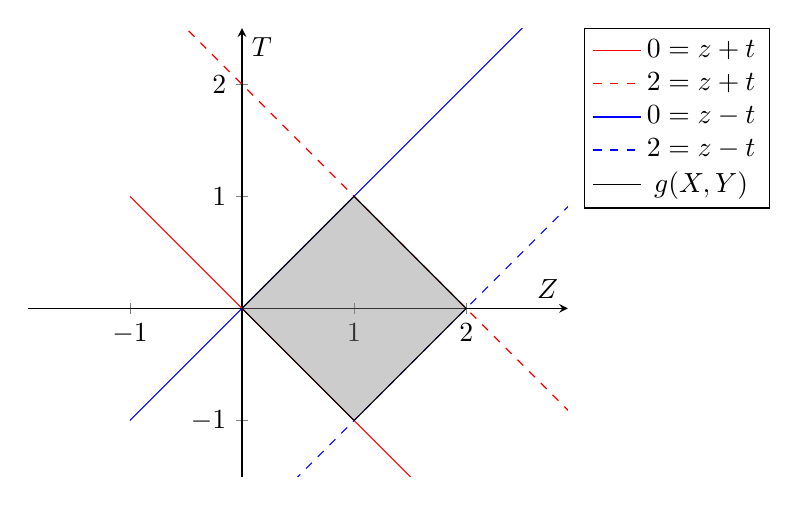
\begin{tikzpicture}
                \begin{axis}[
                    axis lines=middle,
                    xmin=-1.5, xmax=2.5,
                    ymin=-1.5, ymax=2.5,
                    xlabel={$Z$},
                    ylabel={$T$},
                    legend pos=outer north east, % Cambia la posición de la leyenda
                    axis equal,
                ]
                    % Recta 0=z+t
                    \addplot[domain=-1:3, samples=2, color=red]{-x};
                    \addlegendentry{$0=z+t$}
                    % Recta 2=z+t
                    \addplot[domain=-1:3, samples=2, color=red, dashed]{2-x};
                    \addlegendentry{$2=z+t$}
                    % Recta 0=z-t
                    \addplot[domain=-1:3, samples=2, color=blue]{x};
                    \addlegendentry{$0=z-t$}
                    % Recta 2=z-t
                    \addplot[domain=-1:3, samples=2, color=blue, dashed]{x-2};
                    \addlegendentry{$2=z-t$}

                    % Relleno
                    \addplot[fill=gray, fill opacity=0.4] coordinates {(0,0) (1,1) (2,0) (1,-1) (0,0)};
                    \addlegendentry{$g(X,Y)$}

                \end{axis}
            \end{tikzpicture}
        \end{figure}
        
        Buscamos ahora la función de densidad de probabilidad de $(Z,T)$:
        \begin{align*}
            f_{(Z,T)}(z, t)&=f_{(X,Y)}\left(\dfrac{z+t}{2},\dfrac{z-t}{2}\right)\cdot \left|\det Jg^{-1}(z,t)\right|
            =\\&= \begin{cases}
                k\cdot \dfrac{1}{2} & (z,t)\in g(X,Y), \\
                0 & \text{en otro caso}.
            \end{cases}
        \end{align*}

        Por tanto, la función de densidad de probabilidad de $(Z,T)$ es:
        \begin{equation*}
            f_{(Z,T)}(z, t) = \begin{cases}
                \dfrac{1}{2} & 0<z+t<2,~0<z-t<2, \\
                0 & \text{en otro caso}.
            \end{cases}
        \end{equation*}

        \item Determinar las funciones de densidad de probabilidad marginales del vector transformado $(Z,T)$.
        
        Para $z\in [0,2]$, tenemos que:
        \begin{align*}
            f_Z(z)&=\int_{-\infty}^{+\infty} f_{(Z,T)}(z, t) \, dt
        \end{align*}

        Los límites de integración los vemos claros en la gráfica anterior. Distinguimos en función del valor de $z$:
        \begin{itemize}
            \item Si $z\in [0,1]$, entonces:
            \begin{align*}
                f_Z(z)&=\int_{-z}^{z} \dfrac{1}{2} \, dt = \dfrac{1}{2}\left[t\right]_{-z}^z = \dfrac{1}{2}(z-(-z)) = z.
            \end{align*}

            \item Si $z\in [1,2]$, entonces:
            \begin{align*}
                f_Z(z)&=\int_{z-2}^{2-z} \dfrac{1}{2} \, dt = \dfrac{1}{2}\left[t\right]_{z-2}^{2-z} = \dfrac{1}{2}(2-z-(z-2)) = \dfrac{1}{2}(4-2z) = 2-z.
            \end{align*}
        \end{itemize}

        Por tanto, la función de densidad de probabilidad de $Z$ es:
        \begin{equation*}
            f_Z(z) = \begin{cases}
                z & 0<z<1, \\
                2-z & 1<z<2, \\
                0 & \text{en otro caso}.
            \end{cases}
        \end{equation*}

        Para $t\in [-1,1]$, tenemos que:
        \begin{align*}
            f_T(t)&=\int_{-\infty}^{+\infty} f_{(Z,T)}(z, t) \, dz
        \end{align*}

        Los límites de integración los vemos claros en la gráfica anterior. Distinguimos en función del valor de $t$:
        \begin{itemize}
            \item Si $t\in [-1,0]$, entonces:
            \begin{align*}
                f_T(t)&=\int_{-t}^{2+t} \dfrac{1}{2} \, dz = \dfrac{1}{2}\left[z\right]_{-t}^{2+t} = \dfrac{1}{2}(2+t-(-t)) = 1+t.
            \end{align*}

            \item Si $t\in [0,1]$, entonces:
            \begin{align*}
                f_T(t)&=\int_{t}^{2-t} \dfrac{1}{2} \, dz = \dfrac{1}{2}\left[z\right]_{t}^{2-t} = \dfrac{1}{2}(2-t-t) = 1-t.
            \end{align*}
        \end{itemize}

        Por tanto, la función de densidad de probabilidad de $T$ es:
        \begin{equation*}
            f_T(t) = \begin{cases}
                1+t & -1<t<0, \\
                1-t & 0<t<1, \\
                0 & \text{en otro caso}.
            \end{cases}
        \end{equation*}
        

        \item Determinar la función de distribución de probabilidad de $\nicefrac{X}{Y}$ y $XY$.
        % Hasta aquí hecho en clase. Preguntar a Joaquín

        Definimos la transformación:
        \Func{g}{\bb{R}^2}{\bb{R}^2}{(X,Y)}{(Z,T)=(\nicefrac{X}{Y},XY)}

        Para obtener $g^{-1}$, buscamos obtener $X,Y$ en función de $Z,T$:
        \begin{equation*}
            \left\{\begin{aligned}
                Z&=\nicefrac{X}{Y}, \\
                T&=XY.
            \end{aligned}\right\}\Longrightarrow
            \left\{\begin{aligned}
                X&=ZY=\sqrt{ZT}, \\
                Y&=\sqrt{\nicefrac{T}{Z}}.
            \end{aligned}\right.
        \end{equation*}
        Como $X,Y>0$, entonces $Z,T>0$, por lo que la inversa está bien definida.
        \Func{g^{-1}}{\bb{R}^+\times \bb{R}^+}{\bb{R}^2}{(Z,T)}{(X,Y)=(\sqrt{ZT},\sqrt{\nicefrac{T}{Z}})}

        Tenemos que todas las componentes de $g^{-1}$ son derivables:
        \begin{align*}
            \dfrac{\partial X}{\partial Z}(Z,T)&=\dfrac{T}{2\sqrt{ZT}}=\dfrac{\sqrt{T}}{2\sqrt{Z}}, & \dfrac{\partial X}{\partial T}(Z,T)&=\dfrac{\sqrt{Z}}{2\sqrt{T}},\\
            \dfrac{\partial Y}{\partial Z}(Z,T)&=\dfrac{-\frac{T}{Z^2}}{2\sqrt{\nicefrac{T}{Z}}}=-\dfrac{\sqrt{T}}{2Z\sqrt{Z}}, & \dfrac{\partial Y}{\partial T}(Z,T)&=\dfrac{1}{2Z\sqrt{\nicefrac{T}{Z}}}=\dfrac{1}{2\sqrt{TZ}}.
        \end{align*}

        Además, tenemos que:
        \begin{equation*}
            \det Jg^{-1}(z,t)=\begin{vmatrix}
                \dfrac{\sqrt{T}}{2\sqrt{Z}} & \dfrac{\sqrt{Z}}{2\sqrt{T}} \\
                -\dfrac{\sqrt{T}}{2Z\sqrt{Z}} & \dfrac{1}{2\sqrt{TZ}}
            \end{vmatrix}=\dfrac{1}{4Z}+\dfrac{1}{4Z}=\frac{1}{2Z}>0 \qquad \forall (z,t)\in\bb{R}^+\times \bb{R}^+.
        \end{equation*}

        Por tanto, $(Z,T)=g(X,Y)$ es un vector aleatorio continuo. Estudiamos ahora el conjunto $g(X,Y)$:
        \begin{align*}
            g(X,Y)&=\left\{(z,t)\in \bb{R}^+\times \bb{R}^+\mid 0<\sqrt{ZT}<1,~0<\sqrt{\nicefrac{T}{Z}}<1\right\}
            =\\&= \left\{(z,t)\in \bb{R}^+\times \bb{R}^+\mid 0<ZT<1,~0<T<Z\right\}
        \end{align*}

        Veamos el conjunto $g(X,Y)$ gráficamente:
        \begin{figure}[H]
            \centering
            \begin{tikzpicture}
                \begin{axis}[
                    axis lines=middle,
                    xmin=-1.5, xmax=2.5,
                    ymin=-1.5, ymax=2.5,
                    xlabel={$Z$},
                    ylabel={$T$},
                    legend pos=outer north east, % Cambia la posición de la leyenda
                    axis equal,
                ]
                    % Recta 0=z*t
                    \addplot[domain=-2:3, samples=2, color=red, dashed]{0};
                    \draw[red, dashed] (axis cs:0,-3) -- (axis cs:0,3);
                    \addlegendentry{$0=ZT$}
                    % Recta 1=z*t
                    \addplot[domain=-2:3, samples=100, color=red, name path=B]{1/x};
                    \addlegendentry{$1=ZT$}
                    % Recta 0=t
                    \addplot[name path=A, domain=-2:3, samples=2, color=blue, dashed]{0};
                    \addlegendentry{$0=T$}
                    % Recta z=t
                    \addplot[domain=-2:3, samples=2, color=blue, name path=C]{x};
                    \addlegendentry{$T=Z$}

                    % Marca del punto (1,1)
                    \addplot[color=black, mark=*, only marks, forget plot] coordinates {(1,1)};
                    \node[anchor=west] at (axis cs:1,1) {$(1,1)$};

                    % Relleno
                    \addplot [
                        thick,
                        color=orange,
                        fill=orange,
                        fill opacity=0.4
                    ]
                    fill between [
                        of=C and A,
                        soft clip={domain=0:1},
                    ];
                    \addplot [
                        thick,
                        color=orange,
                        fill=orange,
                        fill opacity=0.4
                    ]
                    fill between [
                        of=B and A,
                        soft clip={domain=1:4},
                    ];
                \addlegendentry{$g(X,Y)$}

                \end{axis}
            \end{tikzpicture}
        \end{figure}

        Buscamos ahora la función de densidad de probabilidad de $(Z,T)$:
        \begin{align*}
            f_{(Z,T)}(z, t)&=f_{(X,Y)}\left(\sqrt{ZT},\sqrt{\nicefrac{T}{Z}}\right)\cdot \left|\det Jg^{-1}(z,t)\right|
            =\\&= \begin{cases}
                \dfrac{1}{2z} & (z,t)\in g(X,Y), \\
                0 & \text{en otro caso}.
            \end{cases}
        \end{align*}

        Por tanto, la función de densidad de probabilidad de $(Z,T)$ es:
        \begin{equation*}
            f_{(Z,T)}(z, t) = \begin{cases}
                \dfrac{1}{2z} & 0<ZT<1,~0<T<Z, \\
                0 & \text{en otro caso}.
            \end{cases}
        \end{equation*}

        Para obtener la función de densidad de probabilidad de $Z=\nicefrac{X}{Y}$, tenemos que:
        \begin{align*}
            f_{Z}(z)&=\int_{-\infty}^{+\infty} f_{(Z,T)}(z, t) \, dt
        \end{align*}

        Los límites de integración los vemos claros en la gráfica anterior. Distinguimos en función del valor de $z$:
        \begin{itemize}
            \item Si $z\in [0,1]$, entonces:
            \begin{align*}
                f_Z(z)&=\int_{0}^{z} \dfrac{1}{2z} \, dt = \dfrac{1}{2z}\left[t\right]_{0}^{z} = \dfrac{1}{2z}z = \dfrac{1}{2}.
            \end{align*}

            \item Si $z\in \left[1,+\infty\right[$, entonces:
            \begin{align*}
                f_Z(z)&=\int_{0}^{\nicefrac{1}{z}} \dfrac{1}{2z} \, dt = \dfrac{1}{2z}\left[t\right]_{0}^{\nicefrac{1}{z}} = \dfrac{1}{2z^2}.
            \end{align*}
        \end{itemize}

        Por tanto, la función de densidad de probabilidad de $Z$ es:
        \begin{equation*}
            f_Z(z) = \begin{cases}
                \dfrac{1}{2} & 0<z<1, \\ \\
                \dfrac{1}{2z^2} & 1<z, \\
                0 & \text{en otro caso}.
            \end{cases}
        \end{equation*}

        Para obtener la función de densidad de probabilidad de $T=XY$, tenemos que:
        \begin{align*}
            f_{T}(t)&=\int_{-\infty}^{+\infty} f_{(Z,T)}(z, w) \, dz
        \end{align*}

        Los límites de integración los vemos claros en la gráfica anterior. Para $t\in \left]0,1\right]$, tenemos que:
        \begin{align*}
            f_T(t)&=\int_{t}^{\nicefrac{1}{t}} \dfrac{1}{2z} \, dz = \dfrac{1}{2}\left[\ln(z)\right]_{t}^{\nicefrac{1}{t}} = \dfrac{1}{2}\left[\ln\left(\nicefrac{1}{t}\right)-\ln(t)\right]
            = \dfrac{1}{2}\left[\ln(1)-2\ln(t)\right] = -\ln(t)
        \end{align*}

        Por tanto, la función de densidad de probabilidad de $T$ es:
        \begin{equation*}
            f_T(t) = \begin{cases}
                -\ln(t) & 0<t<1, \\
                0 & \text{en otro caso}.
            \end{cases}
        \end{equation*}

        Una vez tenemos ambas marginales, es fácil obtener la función de distribución de cada una.
        Respecto de $Z$, distinguimos en función del valor de $z$:
        \begin{itemize}
            \item Si $z\in [0,1]$, entonces:
            \begin{align*}
                F_Z(z)&=\int_{-\infty}^{z} f_Z(z) \, dz = \int_{0}^{z} \dfrac{1}{2} \, dz = \dfrac{1}{2}\left[z\right]_{0}^{z} = \dfrac{z}{2}
            \end{align*}

            \item Si $z\in \left[1,+\infty\right[$, entonces:
            \begin{align*}
                F_Z(z)&=\int_{-\infty}^{z} f_Z(z) \, dz = \int_{0}^{1} \dfrac{1}{2} \, dz + \int_{1}^{z} \dfrac{1}{2z^2} \, dz
                = \dfrac{1}{2} - \dfrac{1}{2}\left[\frac{1}{z}\right]_{1}^{z}
                =\\&= \dfrac{1}{2} - \dfrac{1}{2}\left(\frac{1}{z}-1\right)
                = 1-\dfrac{1}{2z}
            \end{align*}        
        \end{itemize}

        Por tanto, la función de distribución de probabilidad de $Z=\nicefrac{X}{Y}$ es:
        \begin{equation*}
            F_Z(z) = \begin{cases}
                \dfrac{z}{2} & 0<z<1, \\ \\
                1-\dfrac{1}{2z} & 1<z, \\
                0 & \text{en otro caso}.
            \end{cases}
        \end{equation*}

        Respecto de $T$, para $t\in \left]0,1\right]$, tenemos que:
        \begin{align*}
            F_T(t)&=\int_{-\infty}^{t} f_T(t) \, dt = \int_{0}^{t} -\ln(t) \, dt = -\left[t\ln(t)-t\right]_{0}^{t} =\\&=
            -t\ln(t)+t +\lim_{t\to 0}t\ln(t) = -t\ln(t)+t
        \end{align*}

        Por tanto, la función de distribución de probabilidad de $T=XY$ es:
        \begin{equation*}
            F_T(t) = \begin{cases}
                0 & t\leq 0, \\
                -t\ln(t)+t & 0<t<1, \\
                1 & 1\leq t, \\
            \end{cases}
        \end{equation*}


        \item Determinar la función de distribución de probabilidad de $\max(X,Y)$, y del $\min(X,Y)$.
        
        Dado $x\in \bb{R}$, tenemos que:
        \begin{equation*}
            P[\max(X,Y)\leq x]=P[X\leq x,Y\leq x] = P[(X,Y)\leq (x,x)]
        \end{equation*}

        Calculamos por tanto dicho valor sabiendo $f_{(X,Y)}$. Para $z\in [0,1]$, tenemos que:
        \begin{align*}
            P[(X,Y)\leq (z,z)]&=\int_{0}^{z}\int_{0}^{z} k \, dy \, dx = k\int_{0}^{z} z \, dx
            = kz\left[x\right]_{0}^{z} = kz^2 = z^2
        \end{align*}

        Por tanto, la función de distribución de probabilidad de $\max(X,Y)$ es:
        \begin{equation*}
            F_{\max(X,Y)}(z) = \begin{cases}
                0 & z\leq 0, \\
                z^2 & 0<z<1, \\
                1 & 1\leq z.
            \end{cases}
        \end{equation*}

        Respecto del $\min(X,Y)$, dado $z\in \bb{R}$, tenemos que:
        \begin{equation*}
            P[\min(X,Y)\leq z]=1-P[\min(X,Y)>z]=1-P[(X,Y)>z]
        \end{equation*}

        Calculamos dicho valor sabiendo $f_{(X,Y)}$. Distinguimos en función de $z$:
        \begin{itemize}
            \item Si $z\leq 0$, entonces $P[(X,Y)>z]=1$.

            \item Si $0<z<1$, entonces:
            \begin{align*}
                P[(X,Y)>z]&=\int_{z}^{1}\int_{z}^{1} k \, dy \, dz = k\int_{z}^{1} (1-z) \, dz
                = k(1-z)\left[x\right]_{z}^{1} = (1-z)^2
            \end{align*}

            \item Si $z\geq 1$, entonces $P[(X,Y)>z]=0$.
        \end{itemize}

        Por tanto, la función de distribución de probabilidad de $\min(X,Y)$ es:
        \begin{equation*}
            F_{\min(X,Y)}(z) = 1-P[(X,Y)>z]=\begin{cases}
                0 & z\leq 0, \\
                1-(1-z)^2 & 0<z<1, \\
                1 & 1\leq z.
            \end{cases}
        \end{equation*}

        \item Determinar la función de distribución de probabilidad conjunta del $\max(X,Y)$, y del $\min(X,Y)$.
        
        Dado $z,t\in \bb{R}$, distinguimos casos:
        \begin{itemize}
            \item Si $z\leq t$, como $\min (X,Y)\leq \max(X,Y)$, entonces:
            \begin{align*}
                P[\max(X,Y)\leq z,\min(X,Y)\leq t]&=P[\max(X,Y)\leq z] = F_{\max(X,Y)}(z)
            \end{align*}

            Distinguimos en función de $z$:
            \begin{itemize}
                \item Si $z\leq 0$, entonces $F_{\max(X,Y)}(z)=0$.
                \item Si $0<z<1$, entonces $F_{\max(X,Y)}(z)=z^2$.
                \item Si $z\geq 1$, entonces $F_{\max(X,Y)}(z)=1$.
            \end{itemize}

            \item Si $z>t$, entonces:
            \begin{align*}
                P[\max(X,Y)\leq z,&\min(X,Y)\leq t]
                \\&=P[\max(X,Y)\leq z]-P[\max(X,Y)\leq z,\min(X,Y)> t]
                =\\&= P[\max(X,Y)\leq z]-P[t<X\leq z,t<Y\leq z]
            \end{align*}

            Distinguimos en función de $z$:
            \begin{itemize}
                \item Si $z\leq 0$, entonces $P[\max(X,Y)\leq z]=0$. Además, $t<z\leq 0$. Por tanto:
                \begin{equation*}
                    P[t<X\leq z,t<Y\leq z]=0
                \end{equation*}
                Por tanto, $P[\max(X,Y)\leq z,\min(X,Y)\leq t]=0$.

                \item Si $0<z<1$, entonces $P[\max(X,Y)\leq z]=z^2$. Además, sabemos que $t<z<1$. Distinguimos en función de $t$:
                \begin{itemize}
                    \item Si $t\leq 0$, entonces:
                    \begin{align*}
                        P[t<X\leq z,t<Y\leq z]&=\int_{0}^{z}\int_{0}^{z} k \, dy \, dx = kz^2 = z^2
                    \end{align*}
                    Por tanto, $P[\max(X,Y)\leq z,\min(X,Y)\leq t]=z^2-z^2=0$.
                    \item Si $0<t<z$, entonces:
                    \begin{align*}
                        P[t<X\leq z,t<Y\leq z]&=\int_{t}^{z}\int_{t}^{z} k \, dy \, dx = k(z-t)^2 = (z-t)^2
                    \end{align*}
                    Por tanto, tenemos que:
                    $$P[\max(X,Y)\leq z,\min(X,Y)\leq t]=z^2-(z-t)^2=z^2-z^2+2zt-t^2=2zt-t^2$$
                \end{itemize}
                \item Si $z\geq 1$, entonces $P[\max(X,Y)\leq z]=1$. Distinguimos en función de $t$:
                \begin{itemize}
                    \item Si $t\leq 0$, entonces:
                    \begin{align*}
                        P[t<X\leq z,t<Y\leq z]&=\int_{0}^{1}\int_{0}^{1} k \, dy \, dx = k = 1
                    \end{align*}
                    Por tanto, $P[\max(X,Y)\leq z,\min(X,Y)\leq t]=1-1=0$.
                    \item Si $0<t<1$, entonces:
                    \begin{align*}
                        P[t<X\leq z,t<Y\leq z]&=\int_{t}^{1}\int_{t}^{1} k \, dy \, dx = k(1-t)^2 = (1-t)^2
                    \end{align*}
                    Por tanto, $$P[\max(X,Y)\leq z,\min(X,Y)\leq t]=1-(1-t)^2=1-1+2t-t^2=2t-t^2$$
                    \item Si $t\geq 1$, $t<z$, entonces:
                    \begin{align*}
                        P[t<X\leq z,t<Y\leq z]&=0
                    \end{align*}
                    Por tanto, $P[\max(X,Y)\leq z,\min(X,Y)\leq t]=1-0=1$.
                \end{itemize}
            \end{itemize}
        \end{itemize}
        
            
        Por tanto, la función de distribución de probabilidad conjunta de $\max(X,Y)$ y $\min(X,Y)$ es:
        \begin{equation*}
            F_{\max(X,Y),\min(X,Y)}(z,t) = \begin{cases}
                0 & z\leq 0 \lor t\leq 0\qquad (R_0), \\
                z^2 & z\leq t \land 0<z<1 \qquad (R_1), \\
                2zt-t^2 & 0<t<z<1 \qquad (R_2), \\
                2t-t^2 & 0<t<1\leq z \qquad (R_3), \\
                1 & 1\leq t\land 1\leq z \qquad (R_4).
            \end{cases}
        \end{equation*}

        Veamos gráficamente cada una de las regiones:
        \begin{figure}[H]
            \centering
            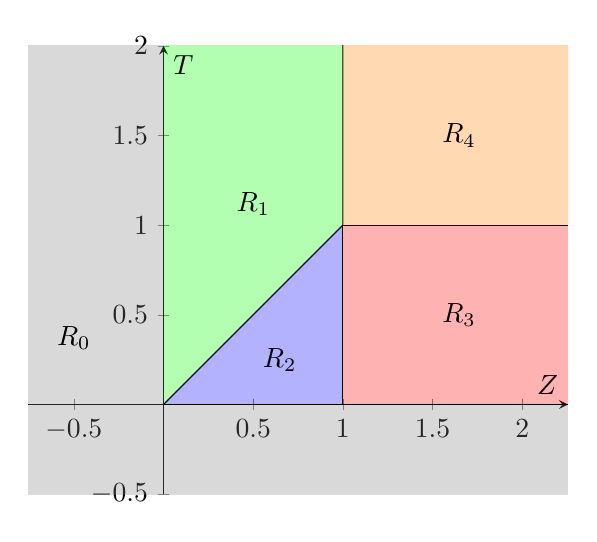
\begin{tikzpicture}
                \begin{axis}[
                    axis lines=middle,
                    xmin=-0.5, xmax=2,
                    ymin=-0.5, ymax=2,
                    xlabel={$Z$},
                    ylabel={$T$},
                    legend pos=outer north east, % Cambia la posición de la leyenda
                    axis equal,
                ]
                    % R0: (0,5) (-5,5) (-5,-5) (5,-5) (5,0) (0,0)
                    \addplot[fill=gray, fill opacity=0.3] coordinates {(0,5) (-5,5) (-5,-5) (5,-5) (5,0) (0,0)};
                    \node[anchor=south] at (-0.5,0.25) {$R_0$};

                    % R1: (0,0) (1,1) (1,5) (0,5)
                    \addplot[fill=green, fill opacity=0.3] coordinates {(0,0) (1,1) (1,5) (0,5)};
                    \node[anchor=south] at (0.5,1) {$R_1$};

                    % R2: (0,0) (1,0) (1,1)
                    \addplot[fill=blue, fill opacity=0.3] coordinates {(0,0) (1,0) (1,1)};
                    \node[anchor=west] at (axis cs:0.5,0.25) {$R_2$};

                    % R3: (1,0) (1,1) (5,1) (5,0)
                    \addplot[fill=red, fill opacity=0.3] coordinates {(1,0) (1,1) (5,1) (5,0)};
                    \node[anchor=west] at (axis cs:1.5,0.5) {$R_3$};

                    % R4: (1,1) (5,1) (5,5) (1,5)
                    \addplot[fill=orange, fill opacity=0.3] coordinates {(1,1) (5,1) (5,5) (1,5)};
                    \node[anchor=west] at (axis cs:1.5,1.5) {$R_4$};
                    
                \end{axis}
            \end{tikzpicture}
        \end{figure}
    \end{enumerate}
\end{ejercicio}

\begin{ejercicio}
    Sea $(X,Y)$ un vector aleatorio bidimensional discreto, cuya función masa de probabilidad conjunta se calcula como el producto de las funciones masa de probabilidad marginales de $X$ e $Y$. Las variables aleatorias $X$ e $Y$ se distribuyen según una Poisson con parámetro $\lambda>0$. Calcular la función de distribución de probabilidad marginal del máximo y del mínimo, así como la distribución conjunta del máximo y del mínimo.\\

    Tenemos que:
    \begin{equation*}
        P[X=x,Y=y] = P[X=x]\cdot P[Y=y]
    \end{equation*}

    Como $X,Y\sim \cc{P}(\lm)$, tenemos que:
    \begin{align*}
        P[X=x,Y=y]&=P[X=x]\cdot P[Y=y]
        =\\&= \dfrac{e^{-\lm}\lm^x}{x!}\cdot \dfrac{e^{-\lm}\lm^y}{y!}
        =\\&= \dfrac{e^{-2\lm}\lm^{x+y}}{x!y!}
    \end{align*}

    Calculemos la marginal del máximo. Para $n\in \bb{N}$, tenemos que:
    \begin{align*}
        P[\max(X,Y)\leq n]&=P[X\leq n,Y\leq n]
        = P[(X,Y)\leq (n,n)]
        =\\&= \sum_{i=0}^{n}\sum_{j=0}^{n}P[X=i,Y=j]
        =\\&= \sum_{i=0}^{n}\sum_{j=0}^{n}\dfrac{e^{-2\lm}\lm^{i+j}}{i!j!}
        =\\&= e^{-2\lm}\sum_{i=0}^{n}\sum_{j=0}^{n}\dfrac{\lm^{i+j}}{i!j!}
        = e^{-2\lm}\sum_{i=0}^{n}\dfrac{\lm^i}{i!}\sum_{j=0}^{n}\dfrac{\lm^j}{j!}
        =\\&= P[X\leq n]\cdot P[Y\leq n]
    \end{align*}

    Calculamos la marginal del mínimo. Para $n\in \bb{N}$, tenemos que:
    \begin{align*}
        P[\min(X,Y)\leq n]&=1-P[\min(X,Y)>n]
        =\\&= 1-P[X>n,Y>n]
        =\\&= 1-P[(X,Y)>(n,n)]
        =\\&= 1-\sum_{i=n+1}^{+\infty}\sum_{j=n+1}^{+\infty}P[X=i,Y=j]
        =\\&= 1-\sum_{i=n+1}^{+\infty}\sum_{j=n+1}^{+\infty}\dfrac{e^{-2\lm}\lm^{i+j}}{i!j!}
        =\\&= 1-e^{-2\lm}\sum_{i=n+1}^{+\infty}\sum_{j=n+1}^{+\infty}\dfrac{\lm^{i+j}}{i!j!}
        =\\&= 1-e^{-2\lm}\sum_{i=n+1}^{+\infty}\dfrac{\lm^i}{i!}\sum_{j=n+1}^{+\infty}\dfrac{\lm^j}{j!}
        =\\&= 1-P[X>n]\cdot P[Y>n]
    \end{align*}

    Calculamos ahora la distribución conjunta del máximo y del mínimo. Para los valores $n,m\in\bb{N}$, tenemos que:
    \begin{itemize}
        \item Si $n\leq m$, entonces:
        \begin{align*}
            P[\max(X,Y)\leq n,\min(X,Y)\leq m]&=P[\max(X,Y)\leq n]
        \end{align*}

        \item Si $m<n$, entonces:
        \begin{align*}
            P[\max(X,Y)&\leq n,\min(X,Y)\leq m]
            =\\&= P[\max(X,Y)\leq n]-P[\max(X,Y)\leq n,\min(X,Y)> m]
            =\\&= P[\max(X,Y)\leq n]-P[m<X\leq n,m<Y\leq n]
            =\\&= P[X\leq n]\cdot P[Y\leq n]-P[m+1\leq X\leq n,m+1<Y\leq n]
        \end{align*}

        Calculamos la probabilidad $P[m+1\leq X\leq n,m+1<Y\leq n]$:
        \begin{align*}
            P[m+1&\leq X\leq n,m+1<Y\leq n]=\sum_{i=m+1}^{n}\sum_{j=m+1}^{n}P[X=i,Y=j]
            =\\&= \sum_{i=m+1}^{n}\sum_{j=m+1}^{n}\dfrac{e^{-2\lm}\lm^{i+j}}{i!j!}
            =\\&= e^{-2\lm}\sum_{i=m+1}^{n}\sum_{j=m+1}^{n}\dfrac{\lm^{i+j}}{i!j!}
            =\\&= \sum_{i=m+1}^{n}e^{-\lm}\dfrac{\lm^i}{i!}\sum_{j=m+1}^{n}e^{-\lm}\dfrac{\lm^j}{j!}
            =\\&= \left(P[X\leq n]-P[X\leq m]\right)\left(P[Y\leq n]-P[Y\leq m]\right)
        \end{align*}

        Por tanto, la distribución conjunta del máximo y del mínimo es:
        \begin{multline*}
            P[\max(X,Y)\leq n,\min(X,Y)\leq m] =\\= \begin{cases}
                P[X\leq n]\cdot P[Y\leq n] & n\leq m, \\
                P[X\leq n]\cdot P[Y\leq n]-\left(P[X\leq n]-P[X\leq m]\right)\left(P[Y\leq n]-P[Y\leq m]\right) & m<n.
            \end{cases}
        \end{multline*}
    \end{itemize}
\end{ejercicio}

\begin{ejercicio}
    Sea $(X,Y)$ un vector aleatorio con función de densidad de probabilidad
    \begin{equation*}
        f(x, y) = \begin{cases}
            2 & 0<x<1,~0<y<x, \\
            0 & \text{en otro caso}.
        \end{cases}
    \end{equation*}
    Calcular la densidad de probabilidad de las variables $Z=aX+bY$, $T=\nicefrac{X}{Y}$, a partir de la densidad de probabilidad conjunta de $(Z,T)=(aX+bY,\nicefrac{X}{Y})$, $a,b>0$.\\

    Definimos la transformación:
    \Func{g}{E_{(X,Y)}}{\bb{R}^2}{(X,Y)}{(Z,T)=(aX+bY,\nicefrac{X}{Y})}

    Para obtener $g^{-1}$, buscamos obtener $X,Y$ en función de $Z,T$:
    \begin{equation*}
        \left\{\begin{aligned}
            Z&=aX+bY, \\
            T&=\nicefrac{X}{Y}.
        \end{aligned}\right\}\Longrightarrow
        \left\{\begin{aligned}
            X&=\dfrac{TZ}{aT+b}, \\
            Y&=\dfrac{Z}{aT+b}.
        \end{aligned}\right.
    \end{equation*}
    Notemos que $a,b>0$, y como $X,Y>0$, entonces $T>0$. Por tanto, $aT+b>0$, por lo que está bien definida la transformación.

    Por tanto, tenemos que:
    \Func{g^{-1}}{g(E_{(X,Y)})}{E_{(X,Y)}}{(Z,T)}{(X,Y)=\left(\dfrac{TZ}{aT+b},\dfrac{Z}{aT+b}\right)}

    Tenemos que todas las componentes de $g^{-1}$ son derivables:
    \begin{align*}
        \dfrac{\partial X}{\partial Z}(Z,T)&=\dfrac{T}{aT+b}, & \dfrac{\partial X}{\partial T}(Z,T)&=\dfrac{bZ}{(aT+b)^2},\\
        \dfrac{\partial Y}{\partial Z}(Z,T)&=\dfrac{1}{aT+b}, & \dfrac{\partial Y}{\partial T}(Z,T)&=\dfrac{-aZ}{(aT+b)^2}.
    \end{align*}

    Además, tenemos que:
    \begin{align*}
        \det Jg^{-1}(z,t)&=\begin{vmatrix}
            \dfrac{T}{aT+b} & \dfrac{bZ}{(aT+b)^2} \\
            \dfrac{1}{aT+b} & \dfrac{-aZ}{(aT+b)^2}
        \end{vmatrix}=\dfrac{1}{(aT+b)^4}\begin{vmatrix}
            T(aT+b) & bZ \\
            aT+b & -aZ
        \end{vmatrix}
        =\\&=\dfrac{1}{(aT+b)^4}(aT+b)(-TaZ -bZ)
        = -\dfrac{Z}{(aT+b)^2}\neq 0 \qquad \forall (z,t)\in g(E_{(X,Y)}).
    \end{align*}

    Por tanto, $(Z,T)=g(X,Y)$ es un vector aleatorio continuo. Veamos ahora el valor de $g(X,Y)$ para $X\in [0,1]$, $Y\in [0,X]$:
    \begin{align*}
        g(X,Y)&=\left\{(z,t)\in \bb{R}^2\mid 0<\dfrac{tz}{at+b}<1,~0<\dfrac{z}{at+b}<\dfrac{tz}{at+b}\right\}
        =\\&= \left\{(z,t)\in \bb{R}^2\mid 0<tz<at+b,~0<1<t\right\}
        =\\&= \left\{(z,t)\in \bb{R}^2\mid 0<z<a+\dfrac{b}{t},~1<t\right\}
    \end{align*}

    Veamos este conjunto gráficamente:
    \begin{figure}[H]
        \centering
        \begin{tikzpicture}
            \begin{axis}[
                axis lines=middle,
                xmin=-1, xmax=4,
                ymin=-1, ymax=4,
                xlabel={$Z$},
                ylabel={$T$},
                xtick=\empty,
                ytick=\empty,
                legend pos=outer north east, % Cambia la posición de la leyenda
                axis equal,
            ]   
                
                % Recta 1=t
                \addplot[name path=A, domain=-3:4, samples=2, color=blue]{1};
                \addlegendentry{$1=t$}
                % Hipérbola y=B/(x-A)
                \addplot[name path=B, domain=1:4, samples=100, color=red]{1/(x-1)};
                \addplot[domain=-3:0.9, samples=100, color=red, forget plot]{1/(x-1)};
                \addlegendentry{$z=a+\nicefrac{b}{t}$}

                % Asíntotas de la hipérbola
                \addplot[domain=-3:4, samples=2, color=red, dashed]{0};
                \draw[dashed, red] (axis cs:1,-2) -- (axis cs:1,4);

                % Indicamos que la asíntota es en z=a y en t=0
                \node[red, right] at (axis cs:1,-0.5) {$z=a$};
                \node[red, above left] at (axis cs:-0.5,0) {$t=0$};

                % Relleno entre la hipérbola y la recta
                \addplot [
                        thick,
                        color=orange,
                        fill=orange,
                        fill opacity=0.4
                    ]
                    fill between [
                        of=B and A,
                        soft clip={domain=1:2},
                    ];
                \addlegendentry{$g(X,Y)$}

                % Señalizamos el punto (a,1) y el punto (a+b,1)
                \node[circle,fill,inner sep=1pt, label=above left:{$(a,1)$}] at (axis cs:1,1) {};
                \node[circle,fill,inner sep=1pt, label=above right:{$(a+b,1)$}] at (axis cs:2,1) {};
            \end{axis}
        \end{tikzpicture}
    \end{figure}    

    La densidad de probabilidad de $(Z,T)$ es:
    \begin{align*}
        &f_{(Z,T)}(z, t) = f_{(X,Y)}\left(\dfrac{tz}{at+b},\dfrac{z}{at+b}\right)\cdot \left|- \dfrac{Z}{(aT+b)^2}\right|
        =\\&= \begin{cases}
            \dfrac{2z}{(at+b)^2} & (z,t)\in g(X,Y), \\
            0 & \text{en otro caso}.
        \end{cases}
    \end{align*}

    Por tanto, la densidad de probabilidad de $(Z,T)$ es:
    \begin{equation*}
        f_{(Z,T)}(z, t) = \begin{cases}
            \dfrac{2z}{(at+b)^2} & (z,t)\in g(X,Y), \\
            0 & \text{en otro caso}.
        \end{cases}
    \end{equation*}

    Calculemos ahora la densidad de probabilidad de $Z=aX+bY$. Para $z\in\left]a,a+b\right[$, tenemos que:
    \begin{align*}
        f_Z(z)&=\int_{-\infty}^{+\infty} f_{(Z,T)}(z, t) \, dt
        = \int_{1}^{\frac{b}{z-a}} \dfrac{2z}{(at+b)^2} \, dt
        =\\&= -\frac{2z}{a}\left[\dfrac{1}{at+b}\right]_{1}^{\frac{b}{z-a}}
        = -\frac{2z}{a}\left[\dfrac{1}{\frac{ba}{z-a}+b}-\dfrac{1}{a+b}\right]
        = -\frac{2z}{a}\left[\dfrac{z-a}{bz}-\dfrac{1}{a+b}\right]
        =\\&= -\frac{2\cancel{z}}{a}\left[\dfrac{(z-a)(a+b)-bz}{b\cancel{z}(a+b)}\right]
        = -\frac{2}{a}\left[\dfrac{az+\cancel{bz}-a^2-ab-\cancel{bz}}{b(a+b)}\right]
        =\\&= 2\cdot \left[\dfrac{a+b-z}{b(a+b)}\right]
    \end{align*}

    Por tanto, la densidad de probabilidad de $Z=aX+bY$ es:
    \begin{equation*}
        f_Z(z) = \begin{cases}
            2\cdot \left[\dfrac{a+b-z}{b(a+b)}\right] & z\in\left]a,a+b\right[, \\
            0 & \text{en otro caso}.
        \end{cases}
    \end{equation*}

    Calculemos ahora la densidad de probabilidad de $T=\nicefrac{X}{Y}$. Para $t>1$, tenemos que:
    \begin{align*}
        f_T(t)&=\int_{-\infty}^{+\infty} f_{(Z,T)}(z, t) \, dz
        = \int_{a}^{a+\frac{b}{t}} \dfrac{2z}{(at+b)^2} \, dz
        =\\&= \dfrac{1}{(at+b)^2}\left[z^2\right]_{a}^{a+\frac{b}{t}}
        = \dfrac{1}{(at+b)^2}\left[\left(a+\dfrac{b}{t}\right)^2-a^2\right]
        =\\&= \dfrac{1}{(at+b)^2}\left[\dfrac{2ab}{t}+\dfrac{b^2}{t^2}\right]
        = \dfrac{b}{(at+b)^2}\left[\dfrac{2at+b}{t^2}\right]
    \end{align*}

    Por tanto, la densidad de probabilidad de $T=\nicefrac{X}{Y}$ es:
    \begin{equation*}
        f_T(t) = \begin{cases}
            \dfrac{b}{(at+b)^2}\left[\dfrac{2at+b}{t^2}\right] & t>1, \\
            0 & \text{en otro caso}.
        \end{cases}
    \end{equation*}


\end{ejercicio}

\begin{ejercicio}
    Sea $(X,Y)$ un vector aleatorio, cuya función de densidad de probabilidad conjunta se calcula como producto de las funciones de densidad de probabilidad marginales de $X$ e $Y$, siendo $X\sim\exp(\lambda)$ e $Y\sim\exp(\mu)$. Calcular la función de distribución de probabilidad conjunta del vector aleatorio
    $$(Z,T)=(\min(X,Y),T),\qquad T=\begin{cases} 0 & Y<X \\ 1 & X<Y \end{cases}$$

    Como $X\sim \exp(\lm)$ e $Y\sim \exp(\mu)$, tenemos que:
    \begin{align*}
        f_X(x)&=\begin{cases}
            \lm e^{-\lm x} & x\geq 0, \\
            0 & x<0,
        \end{cases} & f_Y(y)&=\begin{cases}
            \mu e^{-\mu y} & y\geq 0, \\
            0 & y<0.
        \end{cases}
    \end{align*}

    Por tanto, la función de densidad de probabilidad conjunta de $(X,Y)$ es:
    \begin{align*}
        f_{(X,Y)}(x,y)&=f_X(x)\cdot f_Y(y)
        = \begin{cases}
            \lm\mu e^{-\lm x-\mu y} & x,y\geq 0, \\
            0 & \text{en otro caso}.
        \end{cases}
    \end{align*}

    Tenemos que $E_X=E_Y=\bb{R}^+$, por lo que $E_Z=\bb{R}^+$. Además, $E_T=\{0,1\}$.
    Tenemos por tanto la siguiente situación:
    \begin{figure}[H]
        \centering
        \begin{tikzpicture}
            \begin{axis}[
                axis lines=middle,
                xmin=-1, xmax=4,
                ymin=-1, ymax=2,
                xlabel={$Z$},
                ylabel={$T$},
                legend pos=outer north east, % Cambia la posición de la leyenda
                axis equal,
            ]   
                
                % Recta 1=t
                \addplot[name path=A, domain=-3:4, samples=2, color=blue, thick]{1};
                \addlegendentry{$T=1$}
                % Recta 0=t
                \addplot[name path=B, domain=-3:4, samples=2, color=blue, thick, dashed]{0};
                \addlegendentry{$T=0$}

                % Zona 0:Triángulo (0,0) (0,5) (-5,5) (-5,-5) (5,-5) (5,0)
                \fill[red, opacity=0.2] (0,0) -- (0,5) -- (-5,5) -- (-5,-5) -- (5,-5) -- (5,0) -- cycle;
                \node at (-0.5,-0.5) {$R_0$};

                % Zona 1:Triángulo (0,0) (5,0) (5,1) (0,1)
                \fill[green, opacity=0.2] (0,0) -- (5,0) -- (5,1) -- (0,1) -- cycle;
                \node at (1.5,0.5) {$R_1$};
                
                % Zona 2:Triángulo (0,1) (0,5) (5,5) (5,1)
                \fill[orange, opacity=0.2] (0,1) -- (0,5) -- (5,5) -- (5,1) -- cycle;
                \node at (1.5,1.5) {$R_2$};
            \end{axis}
        \end{tikzpicture}
    \end{figure}

    Calculamos la función de distribución de probabilidad conjunta de $(Z,T)$:
    \begin{align*}
        P[Z\leq z,T\leq t]&=P[\min(X,Y)\leq z,T\leq t]
    \end{align*}

    Dados $z,t\in \bb{R}$, distinguimos casos:
    \begin{itemize}
        \item Si $z\leq 0$ o $t<0$, (es decir, $(z,t)\in R_0$), entonces:
        \begin{equation*}
            P[\min(X,Y)\leq z,T\leq t]=0
        \end{equation*}

        \item Si $z>0$ y $t\in \left[0,1\right[$, (es decir, $(z,t)\in R_1$), entonces:
        \begin{align*}
            P[\min(X,Y)\leq z,T\leq t]&=P[\min(X,Y)\leq z,T=0]
            = P[\min(X,Y)\leq z,Y<X]
            =\\&= P[Y\leq z,Y<X]
            = \int_{0}^{z}\int_{y}^{+\infty} f_{(X,Y)}(x,y) \, dx \, dy
            =\\&= \int_{0}^{z}\int_{y}^{+\infty} \lm\mu e^{-\lm x-\mu y} \, dx \, dy
            = \int_{0}^{z}\mu e^{-\mu y}\int_{y}^{+\infty} \lm e^{-\lm x} \, dx \, dy
            =\\&= \int_{0}^{z}\mu e^{-\mu y}\left[-e^{-\lm x}\right]_{y}^{+\infty} \, dy
            = \int_{0}^{z}\mu e^{-\mu y}e^{-\lm y} \, dy
            =\\&= \mu\int_{0}^{z} e^{-(\lm+\mu)y} \, dy
            = \mu\left[\dfrac{e^{-(\lm+\mu)y}}{-(\lm+\mu)}\right]_{0}^{z}
            =\\&= -\dfrac{\mu}{\lm+\mu} \left[\exp(-(\lm+\mu)z)-1\right]
        \end{align*}

        \item Si $z>0$ y $t\geq 1$, (es decir, $(z,t)\in R_2$), entonces:
        
        Tenemos dos opciones para calcular $P[\min(X,Y)\leq z,T\leq t]$:
        \begin{description}
            \item[Opción 1)] Como $E_T=\{0,1\}$, sabemos que:
            \begin{align*}
                P[\min(X,Y)\leq z,T\leq t]&=P[\min(X,Y)\leq z]
            \end{align*}

            Por tanto, calculamos $P[\min(X,Y)\leq z]$:
            \begin{align*}
                P[\min(X,Y)\leq z] &= 1-P[\min(X,Y)>z] = 1-P[X>z,Y>z]
                =\\&= 1-\int_{z}^{+\infty}\int_{z}^{+\infty} f_{(X,Y)}(x,y) \, dy \, dx
                =\\&= 1-\int_{z}^{+\infty}\int_{z}^{+\infty} \lm\mu e^{-\lm x-\mu y} \, dy \, dx
                =\\&= 1-\int_{z}^{+\infty}\lm e^{-\lm x}\, dx \, \int_{z}^{+\infty} \mu e^{-\mu y} \, dy
                =\\&= 1-\left[-e^{-\lm x}\right]_{z}^{+\infty}\left[-e^{-\mu y}\right]_{z}^{+\infty}
                = 1-\left[e^{-\lm z}-0\right]\left[e^{-\mu z}-0\right]
                =\\&= 1-(e^{-\lm z})(e^{-\mu z})
                = 1-\exp(-(\lm+\mu)z)
            \end{align*}

            \item[Opción 2)] Como $E_T=\{0,1\}$, sabemos que:
            \begin{align*}
                P[\min(X,Y)\leq z,T\leq t]&=P[\min(X,Y)\leq z,T=0] + P[\min(X,Y)\leq z,T=1]
            \end{align*}

            La primera ya la hemos obtenido anteriormente. por tanto, calculamos la segunda probabilidad:
            \begin{align*}
                P[\min(X,Y)\leq z,T=1]&=P[\min(X,Y)\leq z,X<Y] = P[X\leq z,X<Y]
                =\\&= \int_{0}^{z}\int_{x}^{+\infty} f_{(X,Y)}(x,y) \, dy \, dx
                = \int_{0}^{z}\int_{x}^{+\infty} \lm\mu e^{-\lm x-\mu y} \, dy \, dx
                =\\&= \int_{0}^{z}\lm e^{-\lm x}\int_{x}^{+\infty} \mu e^{-\mu y} \, dy \, dx
                = \int_{0}^{z}\lm e^{-\lm x}\left[-e^{-\mu y}\right]_{x}^{+\infty} \, dx
                =\\&= \int_{0}^{z}\lm e^{-\lm x}e^{-\mu x} \, dx
                = \lm\int_{0}^{z} e^{-(\lm+\mu)x} \, dx
                = \lm\left[\dfrac{e^{-(\lm+\mu)x}}{-(\lm+\mu)}\right]_{0}^{z}
                =\\&= -\dfrac{\lm}{\lm+\mu} \left[\exp(-(\lm+\mu)z)-1\right]
            \end{align*}

            Sumando ambos resultados, tenemos que:
            \begin{align*}
                P[\min(X,Y)\leq z,T\leq t]&= [\exp(-(\lm+\mu)z)-1]\left(-\dfrac{\mu}{\lm+\mu} -\dfrac{\lm}{\lm+\mu}\right)
                =\\&= 1-\exp(-(\lm+\mu)z)
            \end{align*}
        \end{description}
    \end{itemize}

    En cualquier caso, la función de distribución de probabilidad conjunta $(Z,T)$ es:
    \begin{equation*}
        F_{(Z,T)}(z,t) = \begin{cases}
            0 & z\leq 0 \text{ o } t<0, \\
            -\dfrac{\mu}{\lm+\mu} \left[\exp(-(\lm+\mu)z)-1\right] & z>0 \text{ y } t\in \left[0,1\right[, \\
            1-\exp(-(\lm+\mu)z) & z>0 \text{ y } t\geq 1.
        \end{cases}
    \end{equation*}
\end{ejercicio}

\begin{ejercicio}
    Sea $(X,Y)$ un vector aleatorio, cuya función de densidad de probabilidad conjunta se calcula como en el problema anterior, considerando $\lambda=\mu$. Calcular la distribución de probabilidad de:
    \begin{enumerate}
        \item $|X-Y|$,

        Del apartado anterior, tenemos que:
        \begin{equation*}
            f_{(X,Y)}(x,y)=\begin{cases}
                \lm^2 e^{-\lm(x+y)} & x,y\geq 0, \\
                0 & \text{en otro caso}.
            \end{cases}
        \end{equation*}

        Buscamos calcular $P[|X-Y|\leq z]$ para todo $z\in\bb{R}$.
        Si $z\leq 0$, tenemos que $P[|X-Y|\leq z]=0$, por lo que sea $z\in \bb{R}^+$.
        Tenemos que:
        \begin{align*}
            P[|X-Y|\leq z]&=P[-z\leq X-Y\leq z]
        \end{align*}

        Sabiendo que $X,Y\geq 0$, tenemos que la situación es la descrita en la Figura~\ref{fig:|X-Y|_z}.
        \begin{figure}
            \centering
            \begin{tikzpicture}
                \begin{axis}[
                    axis lines=middle,
                    xmin=-1, xmax=4,
                    ymin=-1, ymax=4,
                    xlabel={$X$},
                    ylabel={$Y$},
                    legend pos=outer north east, % Cambia la posición de la leyenda
                    axis equal,
                ]
                    % Definimos la variable z>0
                    \def\z{1}
                    
                    % Recta X-Y=-z
                    \addplot[name path=A, domain=-3:4, samples=2, color=blue, thick]{x+\z};
                    \addlegendentry{$X-Y=-z$}
                    % Recta X-Y=z
                    \addplot[name path=B, domain=-3:4, samples=2, color=blue, thick, dashed]{x-\z};
                    \addlegendentry{$X-Y=z$}

                    % Relleno entre las rectas
                    \addplot [
                        thick,
                        color=orange,
                        fill=orange,
                        fill opacity=0.4
                    ]
                    fill between [
                        of=A and B,
                        soft clip={domain=1:4},
                    ];

                    % Relleno (0,0) (0,1) (1,2) (1,0)
                    \fill[orange, opacity=0.4] (0,0) -- (0,1)-- (1,2) -- (1,0) -- cycle;
                    \addlegendentry{$|X-Y|\leq z$,~$X,Y\geq 0$}

                    % Marcamos el punto (z,0)
                    \node[circle,fill,inner sep=1pt, label=above:{$(z,0)$}] at (axis cs:\z,0) {};

                \end{axis}
            \end{tikzpicture}
            \caption{Región de integración para $P[|X-Y|\leq z]$}
            \label{fig:|X-Y|_z}
        \end{figure}

        Por tanto, tenemos que:
        \begin{align*}
            &P[|X-Y|\leq z]=P[-z\leq X-Y\leq z]=\\
            &= \int_{0}^{z}\int_{0}^{x+z} f_{(X,Y)}(x,y) \, dy \, dx
            + \int_{z}^{+\infty}\int_{x-z}^{x+z} f_{(X,Y)}(x,y) \, dy \, dx
            =\\&= \int_{0}^{z}\int_{0}^{x+z} \lm^2 e^{-\lm(x+y)} \, dy \, dx
            + \int_{z}^{+\infty}\int_{x-z}^{x+z} \lm^2 e^{-\lm(x+y)} \, dy \, dx
            =\\&= \int_{0}^{z}\lm e^{-\lm x}\int_{0}^{x+z} \lm e^{-\lm y} \, dy \, dx
            + \int_{z}^{+\infty}\lm e^{-\lm x}\int_{x-z}^{x+z} \lm e^{-\lm y} \, dy \, dx
            =\\&= \int_{0}^{z}\lm e^{-\lm x}\left[-e^{-\lm y}\right]_{0}^{x+z} \, dx
            + \int_{z}^{+\infty}\lm e^{-\lm x}\left[-e^{-\lm y}\right]_{x-z}^{x+z} \, dx
            =\\&= \int_{0}^{z}\lm e^{-\lm x}\left[1-e^{-\lm (x+z)}\right] \, dx
            + \int_{z}^{+\infty}\lm e^{-\lm x}\left[e^{-\lm(x-z)}-e^{-\lm (x+z)}\right] \, dx
            =\\&= \int_{0}^{z} \lm(e^{-\lm x}-e^{-\lm (2x+z)}) \, dx
            + \int_{z}^{+\infty} \lm(e^{-\lm (2x-z)}-e^{-\lm (2x+z)}) \, dx
            =\\&= \left[-e^{-\lm x}+\dfrac{1}{2}e^{-\lm (2x+z)}\right]_{0}^{z}
            + \dfrac{1}{2}\left[-e^{-\lm (2x-z)}+e^{-\lm (2x+z)}\right]_{z}^{+\infty}
            =\\&= -e^{-\lm z}+\cancel{\dfrac{1}{2}e^{-\lm (3z)}}+1-\bcancel{\dfrac{1}{2}e^{-\lm z}}
            + \dfrac{1}{2}\left[0+\bcancel{e^{-\lm (z)}}-\cancel{e^{-\lm (3z)}}\right]
            = 1-e^{-\lm z}
        \end{align*}

        Por tanto, la distribución de probabilidad de $|X-Y|$ es:
        \begin{equation*}
            P[|X-Y|\leq z] = \begin{cases}
                0 & z\leq 0, \\
                1-e^{-\lm z} & z>0.
            \end{cases}
        \end{equation*}

        \item $\max(X,Y^3)$,
        
        Buscamos calcular $P[\max(X,Y^3)\leq z]$ para todo $z\in\bb{R}$.
        \begin{equation*}
            P[\max(X,Y^3)\leq z]=P[X\leq z,Y^3\leq z]
            = P[X\leq z,Y\leq \sqrt[3]{z}]
        \end{equation*}

        Para $z\leq 0$, como $X,Y\geq 0$, tenemos que $P[\max(X,Y^3)\leq z]=0$. Por tanto, sea $z>0$.
        \begin{align*}
            P[\max(X,Y^3)\leq z]&=P[X\leq z,Y\leq \sqrt[3]{z}]
            = \int_{0}^{z}\int_{0}^{\sqrt[3]{z}} f_{(X,Y)}(x,y) \, dy \, dx
            =\\&= \int_{0}^{z}\int_{0}^{\sqrt[3]{z}} \lm^2 e^{-\lm(x+y)} \, dy \, dx
            = \int_{0}^{z}\lm e^{-\lm x} \, dx\int_{0}^{\sqrt[3]{z}} \lm e^{-\lm y} \, dy
            =\\&= \left[-e^{-\lm x}\right]_{0}^{z}\left[-e^{-\lm y}\right]_{0}^{\sqrt[3]{z}}
            = (1-e^{-\lm z})(1-e^{-\lm \sqrt[3]{z}})
        \end{align*}

        Por tanto, la distribución de probabilidad de $\max(X,Y^3)$ es:
        \begin{equation*}
            P[\max(X,Y^3)\leq z] = \begin{cases}
                0 & z\leq 0, \\
                (1-e^{-\lm z})(1-e^{-\lm \sqrt[3]{z}}) & z>0.
            \end{cases}
        \end{equation*}
        \item $\min(X^5,Y)$.
        
        Buscamos calcular $P[\min(X^5,Y)\leq z]$ para todo $z\in\bb{R}$.
        \begin{align*}
            P[\min(X^5,Y)\leq z]&=1-P[\min(X^5,Y)>z]=1-P[X^5>z,Y>z]
            =\\&= 1-P[X>\sqrt[5]{z},Y>z]
        \end{align*}

        Para $z\leq 0$, como $X,Y\geq 0$, tenemos que $P[\min(X^5,Y)\leq z]=0$. Por tanto, sea $z>0$.
        \begin{align*}
            P[\min(X^5,Y)\leq z]&=1-P[X>\sqrt[5]{z},Y>z]
            = 1-\int_{\sqrt[5]{z}}^{+\infty}\int_{z}^{+\infty} f_{(X,Y)}(x,y) \, dy \, dx
            =\\&= 1-\int_{\sqrt[5]{z}}^{+\infty}\int_{z}^{+\infty} \lm^2 e^{-\lm(x+y)} \, dy \, dx
            = 1-\int_{\sqrt[5]{z}}^{+\infty}\lm e^{-\lm x} \, dx\int_{z}^{+\infty} \lm e^{-\lm y} \, dy
            =\\&= 1-\left[-e^{-\lm x}\right]_{\sqrt[5]{z}}^{+\infty}\left[-e^{-\lm y}\right]_{z}^{+\infty}
            = 1-\left[0-e^{-\lm \sqrt[5]{z}}\right]\left[0-e^{-\lm z}\right]
            =\\&= 1-(e^{-\lm \sqrt[5]{z}})(e^{-\lm z})
            = 1-\exp(-\lm(\sqrt[5]{z}+z))
        \end{align*}

        Por tanto, la distribución de probabilidad de $\min(X^5,Y)$ es:
        \begin{equation*}
            P[\min(X^5,Y)\leq z] = \begin{cases}
                0 & z\leq 0, \\
                1-\exp(-\lm(\sqrt[5]{z}+z)) & z>0.
            \end{cases}
        \end{equation*}
    \end{enumerate}
\end{ejercicio}

\begin{ejercicio}
    Sea $(X,Y)$ un vector aleatorio discreto con función masa de probabilidad
    \begin{equation*}
        P[X=x,Y=y] = \dfrac{k}{2^{x+y}},\qquad x,y\in\bb{N}
    \end{equation*}
    \begin{observacion}
        Consideramos $\bb{N}=\bb{N}\cup \{0\}$.
    \end{observacion}
    \begin{enumerate}
        \item Calcular el valor de $k$ para que la ecuación anterior defina la función masa de probabilidad de un variable aleatoria bidimensional discreta.
        
        Tenemos que la suma de una serie geométrica de razón $r\in\left]-1,1\right[$ es:
        \begin{equation*}
            \sum_{n=0}^{+\infty} r^n = \dfrac{1}{1-r}
        \end{equation*}
        
        Para que la función masa de probabilidad sea válida, tenemos que:
        \begin{align*}
            1&=\sum_{x,y=0}^{+\infty} P[X=x,Y=y] = \sum_{x,y=0}^{+\infty} \dfrac{k}{2^{x+y}}
            = k\sum_{x=0}^{+\infty}\dfrac{1}{2^x}\sum_{y=0}^{+\infty}\dfrac{1}{2^y}
            =\\&= k\cdot \dfrac{1}{1-\nicefrac{1}{2}}\cdot \dfrac{1}{1-\nicefrac{1}{2}}
            = k\cdot 2\cdot 2 = 4k
            \Longrightarrow k=\dfrac{1}{4}
        \end{align*}
        \item Calcular las funciones masa de probabilidad marginales y condicionadas.
        
        La función masa de probabilidad marginal de $X$ es:
        \begin{align*}
            P[X=x]&=\sum_{y=0}^{+\infty} P[X=x,Y=y]
            = \sum_{y=0}^{+\infty} \dfrac{1}{4\cdot 2^{x+y}}
            = \dfrac{1}{4}\sum_{y=0}^{+\infty} \dfrac{1}{2^{x+y}}
            =\\&= \dfrac{1}{4}\sum_{y=0}^{+\infty} \dfrac{1}{2^x}\dfrac{1}{2^y}
            = \dfrac{1}{4}\dfrac{1}{2^x}\sum_{y=0}^{+\infty} \dfrac{1}{2^y}
            = \dfrac{1}{4}\dfrac{1}{2^x}\dfrac{1}{1-\nicefrac{1}{2}}
            = \dfrac{1}{4}\dfrac{1}{2^x}\dfrac{1}{\nicefrac{1}{2}}
            = \dfrac{1}{2^{x+1}}
        \end{align*}

        De forma análoga, la función masa de probabilidad marginal de $Y$ es:
        \begin{equation*}
            P[Y=y]=\dfrac{1}{2^{y+1}}
        \end{equation*}

        La función masa de probabilidad condicionada de $X$ dado $Y=y^*\in \bb{N}$ es:
        \begin{align*}
            P[X=x\mid Y=y^*]&=\dfrac{P[X=x,Y=y^*]}{P[Y=y^*]}
            = \dfrac{\frac{1}{4\cdot 2^{x+y^*}}}{\frac{1}{2^{y^*+1}}}
            = \dfrac{1}{4\cdot 2^{x+y^*}}\cdot \dfrac{2^{y^*+1}}{1}
            =\\&= \dfrac{2^{y^*-1}}{2^{x+y^*}}
            = 2^{-(x+1)} \qquad \forall x\in\bb{N}
        \end{align*}

        La función masa de probabilidad condicionada de $Y$ dado $X=x^*\in \bb{N}$ es análoga, y es:
        \begin{equation*}
            P[Y=y\mid X=x^*]=2^{-(y+1)} \qquad \forall y\in\bb{N}
        \end{equation*}
        \item Calcular la función masa de probabilidad de $X+Y$.
        
        Notamos $Z=X+Y$. Definimos las transformación:
        \Func{g}{\bb{R}^2}{\bb{R}}{(X,Y)}{Z=X+Y}
        
        Como $Z=X+Y$, y $X,Y\in\bb{N}$, tenemos que $Z\in\bb{N}$. Busquemos la función masa de probabilidad de $Z$:
        \begin{align*}
            P[Z=z]&=\sum_{\substack{x,y\in\bb{N} \\ x+y=z}} P[X=x,Y=y]
            = \sum_{\substack{x,y\in\bb{N} \\ x+y=z}} \dfrac{1}{4\cdot 2^{x+y}}
            = \sum_{x=0}^{z}\dfrac{1}{4\cdot 2^{x+z-x}}
            = \sum_{x=0}^{z}\dfrac{1}{4\cdot 2^{z}}
            =\\&=\dfrac{z+1}{4\cdot 2^z}
        \end{align*}
        
        \item Calcular la función masa de probabilidad de $X-Y$.
        
        Notamos $T=X-Y$. Definimos las transformación:
        \Func{h}{\bb{R}^2}{\bb{R}}{(X,Y)}{T=X-Y}

        Como $T=X-Y$, y $X,Y\in\bb{N}$, tenemos que $T\in\bb{Z}$. Busquemos la función masa de probabilidad de $T$:
        \begin{align*}
            P[T=t]&=\sum_{\substack{x,y\in\bb{N} \\ x-y=t}} P[X=x,Y=y]
            = \sum_{\substack{x,y\in\bb{N} \\ x-y=t}} \dfrac{1}{4\cdot 2^{x+y}}
            = \sum_{x=0}^{+\infty}\dfrac{1}{4\cdot 2^{x+x-t}}
            = \dfrac{1}{4}\sum_{x=0}^{+\infty}\dfrac{1}{2^{2x-t}}
            =\\&= \dfrac{1}{4\cdot 2^{-t}}\sum_{x=0}^{+\infty}\dfrac{1}{4^x}
            = \dfrac{1}{4\cdot 2^{-t}}\dfrac{1}{1-\nicefrac{1}{4}}
            = \dfrac{1}{4\cdot 2^{-t}}\dfrac{1}{\nicefrac{3}{4}}
            = \dfrac{1}{3\cdot 2^{-t}}
        \end{align*}
    \end{enumerate}
\end{ejercicio}

\begin{ejercicio}
    El vector aleatorio $(X,Y)$ se distribuye según una uniforme sobre el recinto
    \begin{equation*}
        R_1 = \{(x, y); 0<x<y<1\}.
    \end{equation*}
    Calcular:
    \begin{enumerate}
        \item Su función generatriz de momentos conjunta.
        
        Veamos en primer lugar el conjunto $R_1$:
        \begin{figure}[H]
            \centering
            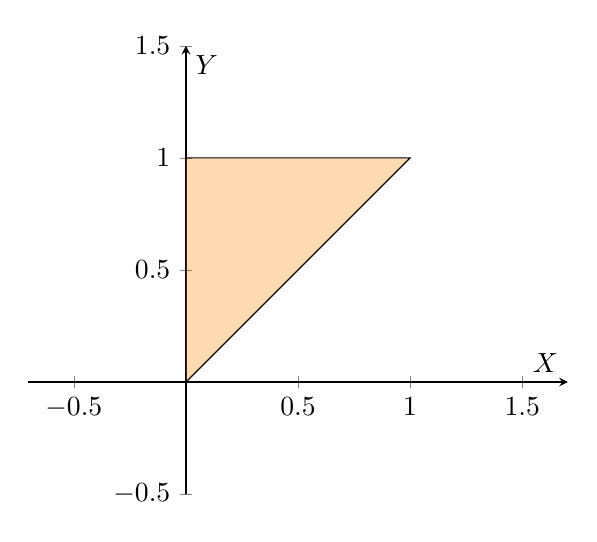
\begin{tikzpicture}
                \begin{axis}[
                    axis lines=middle,
                    xmin=-0.5, xmax=1.5,
                    ymin=-0.5, ymax=1.5,
                    xlabel={$X$},
                    ylabel={$Y$},
                    legend pos=outer north east, % Cambia la posición de la leyenda
                    axis equal,
                ]
                    
                % (0,0) (1,1) (0,1)
                \addplot[fill=orange, fill opacity=0.3] coordinates {(0,0) (1,1) (0,1)};
                \end{axis}
            \end{tikzpicture}
        \end{figure}

        Veamos ahora la función de densidad. Como se distribuye uniformemente, tenemos que:
        \begin{equation*}
            f_{(X,Y)}(x,y)=\begin{cases}
                k & (x,y)\in R_1, \\
                0 & \text{en otro caso}.
            \end{cases}
        \end{equation*}

        Para obtener el valor de $k$, tenemos que:
        \begin{align*}
            1&=\int_{0}^{1}\int_{x}^{1} k \, dy \, dx
            = k\int_{0}^{1}(1-x) \, dx
            = k\left[x-\dfrac{x^2}{2}\right]_{0}^{1}
            = k\left[1-\dfrac{1}{2}\right]
            = \dfrac{k}{2}
            \Longrightarrow k=2
        \end{align*}

        Por tanto, la función de densidad de probabilidad conjunta es:
        \begin{equation*}
            f_{(X,Y)}(x,y)=\begin{cases}
                2 & 0<x<y<1, \\
                0 & \text{en otro caso}.
            \end{cases}
        \end{equation*}

        La función generatriz de momentos conjunta es:
        \begin{align*}
            M_{(X,Y)}(t_1,t_2)&=E[e^{t_1X+t_2Y}]
            = \int_{0}^{1}\int_{x}^{1} e^{t_1x+t_2y} f_{(X,Y)}(x,y) \, dy \, dx
            =\\&= 2\int_{0}^{1}\int_{x}^{1} e^{t_1x+t_2y} \, dy \, dx
            = 2\int_{0}^{1} e^{t_1x}\int_{x}^{1} e^{t_2y} \, dy \, dx
            =\\&= 2\int_{0}^{1} e^{t_1x}\left[\dfrac{e^{t_2y}}{t_2}\right]_{x}^{1} \, dx
            = 2\int_{0}^{1} e^{t_1x}\left[\dfrac{e^{t_2}-e^{t_2x}}{t_2}\right] \, dx
            =\\&= \dfrac{2}{t_2}\int_{0}^{1} e^{t_1x+t_2}-e^{(t_1+t_2)x} \, dx
            = \dfrac{2}{t_2}\left[\dfrac{e^{t_1x+t_2}}{t_1}-\dfrac{e^{(t_1+t_2)x}}{t_1+t_2}\right]_{0}^{1}
            =\\&= \dfrac{2}{t_2}\left[\dfrac{e^{t_1+t_2}}{t_1}-\dfrac{e^{t_1+t_2}}{t_1+t_2}-\dfrac{e^{t_2}}{t_1}+\dfrac{1}{t_1+t_2}\right]
            = \dfrac{2}{t_2}\left[\dfrac{e^{t_1+t_2}-e^{t_2}}{t_1}-\dfrac{e^{t_1+t_2}-1}{t_1+t_2}\right]
        \end{align*}

        Como no podemos evaluar en el origen, sería necesario ver si la función generatriz de momentos es continua en el origen. Para ello, es necesario calcular:
        \begin{equation*}
            \lim_{(t_1,t_2)\to (0,0)} M_{(X,Y)}(t_1,t_2)
        \end{equation*}
        Este límite en varias variables es objetivo de estudio de Análisis, escapándose a los conocimientos de esta asignatura.
        \item Las distribuciones generatrices de momentos marginales.
        \item La covarianza de $X$ e $Y$.
        
        La covarianza de $X$ e $Y$ es:
        \begin{align*}
            \Cov(X,Y)&=E[XY]-E[X]E[Y]
        \end{align*}

        Calculamos cada una de las esperanzas:
        \begin{align*}
            E[X] &= \int_{0}^{1} xf_X(x) \, dx
            = \int_{0}^{1}x \int_{x}^{1} 2 \, dy \, dx
            = 2\int_{0}^{1}x(1-x) \, dx
            = 2\left[\dfrac{x^2}{2}-\dfrac{x^3}{3}\right]_{0}^{1}
            =\\&= 2\left[\dfrac{1}{2}-\dfrac{1}{3}\right]
            = \dfrac{1}{3} \\
            E[Y] &= \int_{0}^{1} yf_Y(y) \, dy
            = \int_{0}^{1}y \int_{0}^{y} 2 \, dx \, dy
            = 2\int_{0}^{1}y^2 \, dy
            = 2\left[\dfrac{y^3}{3}\right]_{0}^{1}
            = \dfrac{2}{3} \\
            E[XY] &= \int_{0}^{1}\int_{x}^{1} xyf_{(X,Y)}(x,y) \, dy \, dx
            = 2\int_{0}^{1}x \int_{x}^{1} y \, dy \, dx
            = 2\int_{0}^{1}x\left[\dfrac{y^2}{2}\right]_{x}^{1} \, dx
            =\\&= 2\int_{0}^{1}x\left[\dfrac{1}{2}-\dfrac{x^2}{2}\right] \, dx
            = 2\int_{0}^{1}\left[\dfrac{x}{2}-\dfrac{x^3}{2}\right] \, dx
            = 2\left[\dfrac{x^2}{4}-\dfrac{x^4}{8}\right]_{0}^{1}
            =\\&= 2\left[\dfrac{1}{4}-\dfrac{1}{8}\right]
            = \dfrac{1}{4}
        \end{align*}

        Por tanto, la covarianza de $X$ e $Y$ es:
        \begin{align*}
            \Cov(X,Y)&=E[XY]-E[X]E[Y]
            = \dfrac{1}{4}-\dfrac{1}{3}\cdot\dfrac{2}{3}
            = \dfrac{1}{4}-\dfrac{2}{9}
            = \dfrac{1}{36}
        \end{align*}
    \end{enumerate}
\end{ejercicio}